\chapter{Results}
\label{chapter6}

The focus of this current chapter is to propose and describe the results obtained, regarding the network CAPEX, for both the analytical and the heuristic models here proposed and the ILP model used from a previous dissertation. Additionally, a comparative study of the algorithms performance in terms of speed was also elaborated. The chapter is mainly divided into two subsections, subsection \ref{ref} contains the results correspondent to the study of reference network, considering the traffic scenarios designed in section \ref{referenceNetwork}, and in subsection \ref{heu} related to the realistic network. Although in section \ref{ref} the results are present for all considered models (analytical, ILP and heuristic), in the particular case of the heuristic model are drawn some specific conclusions regarding the cost per Gbit/s between other aspects. In the end of each section a comparative analysis is provided between the results obtained through the different previously mentioned models. Once again, it is important to alert that only the transparent transport mode without survivability is considered.



\section{Reference Network}
\label{ref}
\vspace{11pt}
In this section are presented the results related to the CAPEX values of the reference network for the low, medium and high traffic scenarios regarding the different considered methods, namely the analytical, the ILP and the heuristic models. At the end, a comparison is made between the values obtained with each method for each traffic scenario and some conclusions are elaborated.

\subsection{Analytical}
\vspace{11pt}
For this specific model all the necessary formulas to obtain the CAPEX value are presented in section \ref{anal}. Moreover, for every scenario the survivability coefficient is considered to be zero since there is no survivability and the grooming coefficient assumes the value 1.25.

\subsubsection{Low traffic}

\vspace{11pt}
In this scenario it has to be taken into account the traffic assumed in subsection \ref{low}.\\

Using equation \ref{demands}:\\

$D$ = ${\frac{1}{2}} \times {( 1 + 1.25 )} \times ( \frac{2000}{100} )$ \qquad \qquad $D$ = 22.5\\

Replacing in equation \ref{optical_channels}:\\

$<w>$ = $(\frac{22.5 \times 1.533}{16} ) \times ( 1 + 0)$ \qquad \qquad $<w>$ = 2.156\\
%$<w>$ = $($ $\frac{22.5 x 1.533}{16}$ $)$ x $($ 1 + 0$)$ \qquad \qquad $<w>$ = 2.156\\

Through equation \ref{amplifiers}:\\

$N^R$ = 16\\

Finally, substituting all these values in equation \ref{analytical_linkCosts} the Link Cost obtained is:\\

$C_L$ = $(2 \times 8 \times 15 000) + (2 \times 8 \times 5 000 \times 2.156) + (2 \times 16 \times 2000)$ = \textbf{476 480 \euro}\\

In relation to the cost of the nodes firstly the average number of demands is calculated as it follows:\\

$<d>$ = $\frac{22.5}{6}$ \qquad \qquad $<d>$ = 3.75\\

Replacing in equations \ref{Pexc_transp} and \ref{Poxc_transp}:\\

$<P_{exc}>$ = 3.75\\

$<P_{oxc}>$ = $3.75 \times [1 + (1 + 0 ) \times 1.533]$ \qquad \quad $<P_{oxc}>$ = 9.4988 \\

Finally, replacing all these values in equations \ref{analytical_electricalCost} and \ref{analytical_opticalCost} the Node Cost is:\\

%$C_N$ = $(1000 \times 100 \times 3.75)$

$C_N$ = $(6 \times (10 000 + (1 00 \times 100 \times 3.75)) + (100 \times 1.25 \times 120) + (100 \times 2.5 \times 100) + (100 \times 10 \times 32) + (100 \times 40 \times 12) + (100 \times 100 \times 8)) + (6 \times (20 000 + (2 500 \times 9.4988 )))$\\

$C_N$ = 485 000 + 262 482 = \textbf{747 482 \euro}\\

$CAPEX$ = 476 480 + 747 482 \qquad \qquad $CAPEX$ = \textbf{1 223 962 \euro}\\


\subsubsection{Medium traffic}
\vspace{11pt}
In this scenario it has to be taken into account the traffic assumed in subsection \ref{medium}.\\

Using equation \ref{demands}:\\

$D$ = ${\frac{1}{2}} \times {( 1 + 1.25 )} \times ( \frac{10000}{100} )$ \qquad \qquad $D$ = 112.5\\

Replacing in equation \ref{optical_channels}:\\

$<w>$ = $(\frac{112.5 \times 1.533}{16} ) \times ( 1 + 0)$ \qquad \qquad $<w>$ = 10.8125\\
%$<w>$ = $($ $\frac{22.5 x 1.533}{16}$ $)$ x $($ 1 + 0$)$ \qquad \qquad $<w>$ = 2.156\\

Through equation \ref{amplifiers}:\\

$N^R$ = 16\\

Finally, substituting all these values in equation \ref{analytical_linkCosts} the Link Cost obtained is:\\

$C_L$ = $(2 \times 8 \times 15 000) + (2 \times 8 \times 5 000 \times 10.8125) + (2 \times 16 \times 2000)$ = \textbf{1 169 000 \euro}\\

In relation to the cost of the nodes firstly the average number of demands is calculated as it follows:\\

$<d>$ = $\frac{112.5}{6}$ \qquad \qquad $<d>$ = 18.75\\

Replacing in equations \ref{Pexc_transp} and \ref{Poxc_transp}:\\

$<P_{exc}>$ = 18.75\\

$<P_{oxc}>$ = $18.75 \times [1 + (1 + 0 ) \times 1.533]$ \qquad \quad $<P_{oxc}>$ = 47.4938 \\

Finally, replacing all these values in equations \ref{analytical_electricalCost} and \ref{analytical_opticalCost} the Node Cost is:\\

%$C_N$ = $(1000 \times 100 \times 3.75)$

$C_N$ = $(6 \times (10 000 + (1 00 \times 100 \times 18.75)) + (100 \times 1.25 \times 600) + (100 \times 2.5 \times 500) + (100 \times 10 \times 160) + (100 \times 40 \times 60) + (100 \times 100 \times 40)) + (6 \times (20 000 + (2 500 \times 47.4938 )))$\\

$C_N$ = 2 185 000 + 832 407 = \textbf{3 017 407 \euro}\\

$CAPEX$ = 1 169 000 + 3 017 407 \qquad \qquad $CAPEX$ = \textbf{4 186 407 \euro}\\

\subsubsection{High traffic}
\vspace{11pt}
In this scenario it has to be taken into account the traffic assumed in subsection \ref{high}.\\

Using equation \ref{demands}:\\

$D$ = ${\frac{1}{2}} \times {( 1 + 1.25 )} \times ( \frac{20000}{100} )$ \qquad \qquad $D$ = 225\\

Replacing in equation \ref{optical_channels}:\\

$<w>$ = $(\frac{225 \times 1.533}{16} ) \times ( 1 + 0)$ \qquad \qquad $<w>$ = 21.5625\\
%$<w>$ = $($ $\frac{22.5 x 1.533}{16}$ $)$ x $($ 1 + 0$)$ \qquad \qquad $<w>$ = 2.156\\

Through equation \ref{amplifiers}:\\

$N^R$ = 16\\

Finally, substituting all these values in equation \ref{analytical_linkCosts} the Link Cost obtained is:\\

$C_L$ = $(2 \times 8 \times 15 000) + (2 \times 8 \times 5 000 \times 21.5625) + (2 \times 16 \times 2000)$ = \textbf{2 029 000 \euro}\\

In relation to the cost of the nodes firstly the average number of demands is calculated as it follows:\\

$<d>$ = $\frac{225}{6}$ \qquad \qquad $<d>$ = 37.5\\

Replacing in equations \ref{Pexc_transp} and \ref{Poxc_transp}:\\

$<P_{exc}>$ = 37.5\\

$<P_{oxc}>$ = $37.5 \times [1 + (1 + 0 ) \times 1.533]$ \qquad \quad $<P_{oxc}>$ = 94.9875 \\

Finally, replacing all these values in equations \ref{analytical_electricalCost} and \ref{analytical_opticalCost} the Node Cost is:\\

%$C_N$ = $(1000 \times 100 \times 3.75)$

$C_N$ = $(6 \times (10 000 + (1 00 \times 100 \times 37.5)) + (100 \times 1.25 \times 600) + (100 \times 2.5 \times 500) + (100 \times 10 \times 160) + (100 \times 40 \times 60) + (100 \times 100 \times 40)) + (6 \times (20 000 + (2 500 \times 94.9875 )))$\\

$C_N$ = 4 310 000 + 1 544 800 = \textbf{5 854 800 \euro}\\

$CAPEX$ = 2 029 000 + 5 854 800 \qquad \qquad $CAPEX$ = \textbf{7 883 800 \euro}\\

Below, in table \ref{analComparison} are summarize the analytical parameters calculated for each traffic scenario.

\begin{table}[H]
\centering
\begin{tabular}{|c|c|c|c|}
\hline
 & \textbf{Low} & \textbf{Medium} & \textbf{High} \\ \hline
$<w>$ & 2.156 & 10.8125 & 21.5625 \\ \hline
$N$ & 16 & 16 & 16 \\ \hline
$<d>$ & 3.75 & 18.75 & 37.5 \\ \hline
$P_{exc}$ & 3.75 & 18.75 & 37.5 \\ \hline
$P_{oxc}$ & 9.4988 & 47.4938 & 94.9875 \\ \hline
$C_{L}$ & 476 480 \euro & 1 169 000 \euro & 2 0 29 000 \euro \\ \hline
$C_{N}$ & 747 482 \euro & 3 017 407 \euro & 5 854 000 \euro \\ \hline
$C_{C}$ & 1 223 962 \euro & 4 186 407 \euro & 7 883 000 \euro \\ \hline
\end{tabular}
\caption{Table containing the analytical estimations for the CAPEX in each traffic scenario.}
\label{analComparison}
\end{table}

\subsection{ILP}

This section contains the obtained CAPEX values for the different traffic scenarios recurring to an ILP model from a previous dissertation \cite{TiagoEsteves}. The type of components, as well its quantity and unity price are also presented. Finally, the cost of the links and also of the nodes is calculated in order to obtain the total cost of the network.

\subsubsection{Low traffic}

\begin{table}[H]
\centering
\scalebox{0.81}{
\begin{tabular}{|c|c|c|c|c|c|c|}
\hline
\multicolumn{7}{|c|}{Network CAPEX} \\ \hline
\multicolumn{3}{|c|}{} & Quantity & Unit Price & Cost & Total \\ \hline
\multirow{3}{*}{\begin{tabular}[c]{@{}c@{}}Link\\ Cost\end{tabular}} & \multicolumn{2}{c|}{OLTs} & 16 & 15 000 \euro & 240 000 \euro & \multirow{3}{*}{584 000 \euro} \\ \cline{2-6}
 & \multicolumn{2}{c|}{Optical Channels} & 56 & 5000 \euro & 280 000 \euro &  \\ \cline{2-6}
 & \multicolumn{2}{c|}{Amplifiers} & 32 & 2000 \euro & 64 000 \euro &  \\ \hline
\multirow{10}{*}{\begin{tabular}[c]{@{}c@{}}Node\\ Cost\end{tabular}} & \multirow{7}{*}{Electrical} & EXCs & 6 & 10 000 \euro & 60 000 \euro & \multirow{10}{*}{1 020 000 \euro} \\ \cline{3-6}
 &  & ODU0 Ports & 120 & 100 \euro/Gbit/s & 15 000 \euro &  \\ \cline{3-6}
 &  & ODU1 Ports & 100 & 100 \euro/Gbit/s & 25 000 \euro &  \\ \cline{3-6}
 &  & ODU2 Ports & 32 & 100 \euro/Gbit/s & 32 000 \euro &  \\ \cline{3-6}
 &  & ODU3 Ports & 12 & 100 \euro/Gbit/s & 48 000 \euro &  \\ \cline{3-6}
 &  & ODU4 Ports & 8 & 100 \euro/Gbit/s & 80 000 \euro &  \\ \cline{3-6}
 &  & LR Transponders & 40 & 100 \euro/Gbit/s & 400 000 \euro &  \\ \cline{2-6}
 & \multirow{3}{*}{Optical} & OXCs & 6 & 20 000 \euro & 120 000 \euro &  \\ \cline{3-6}
 &  & \multirow{2}{*}{OXC Ports} & \multirow{2}{*}{96} & \multirow{2}{*}{2 500 \euro} & \multirow{2}{*}{240 000 \euro} &  \\
 &  &  &  &  &  &  \\ \hline
\multicolumn{6}{|c|}{Total Network Cost} & 1 604 000 \euro \\ \hline
\end{tabular}}
\caption{Detailed description of CAPEX for low traffic scenario using ILPs.}
\end{table}

\subsubsection{Medium traffic}

\begin{table}[H]
\centering
\scalebox{0.81}{
\begin{tabular}{|c|c|c|c|c|c|c|}
\hline
\multicolumn{7}{|c|}{Network CAPEX} \\ \hline
\multicolumn{3}{|c|}{} & Quantity & Unit Price & Cost & Total \\ \hline
\multirow{3}{*}{\begin{tabular}[c]{@{}c@{}}Link\\ Cost\end{tabular}} & \multicolumn{2}{c|}{OLTs} & 16 & 15 000 \euro & 240 000 \euro & \multirow{3}{*}{1 004 000 \euro} \\ \cline{2-6}
 & \multicolumn{2}{c|}{Optical Channels} & 140 & 5000 \euro & 700 000 \euro &  \\ \cline{2-6}
 & \multicolumn{2}{c|}{Amplifiers} & 32 & 2000 \euro & 64 000 \euro &  \\ \hline
\multirow{10}{*}{\begin{tabular}[c]{@{}c@{}}Node\\ Cost\end{tabular}} & \multirow{7}{*}{Electrical} & EXCs & 6 & 10 000 \euro & 60 000 \euro & \multirow{10}{*}{2 955 000 \euro} \\ \cline{3-6}
 &  & ODU0 Ports & 600 & 100 \euro/Gbit/s & 75 000 \euro &  \\ \cline{3-6}
 &  & ODU1 Ports & 500 & 100 \euro/Gbit/s & 125 000 \euro &  \\ \cline{3-6}
 &  & ODU2 Ports & 160 & 100 \euro/Gbit/s & 160 000 \euro &  \\ \cline{3-6}
 &  & ODU3 Ports & 60 & 100 \euro/Gbit/s & 240 000 \euro &  \\ \cline{3-6}
 &  & ODU4 Ports & 40 & 100 \euro/Gbit/s & 400 000 \euro &  \\ \cline{3-6}
 &  & LR Transponders & 114 & 100 \euro/Gbit/s & 1 140 000 \euro &  \\ \cline{2-6}
 & \multirow{3}{*}{Optical} & OXCs & 6 & 20 000 \euro & 120 000 \euro &  \\ \cline{3-6}
 &  & \multirow{2}{*}{OXC Ports} & \multirow{2}{*}{254} & \multirow{2}{*}{2 500 \euro} & \multirow{2}{*}{635 000 \euro} &  \\
 &  &  &  &  &  &  \\ \hline
\multicolumn{6}{|c|}{Total Network Cost} & 3 959 000 \euro \\ \hline
\end{tabular}}
\caption{Detailed description of CAPEX for medium traffic scenario using ILPs.}
\end{table}

\subsubsection{High traffic}

\begin{table}[H]
\centering
\scalebox{0.8}{
\begin{tabular}{|c|c|c|c|c|c|c|}
\hline
\multicolumn{7}{|c|}{Network CAPEX} \\ \hline
\multicolumn{3}{|c|}{} & Quantity & Unit Price & Cost & Total \\ \hline
\multirow{3}{*}{\begin{tabular}[c]{@{}c@{}}Link\\ Cost\end{tabular}} & \multicolumn{2}{c|}{OLTs} & 16 & 15 000 \euro & 240 000 \euro & \multirow{3}{*}{1 604 000 \euro} \\ \cline{2-6}
 & \multicolumn{2}{c|}{Optical Channels} & 260 & 5000 \euro & 1 300 000 \euro &  \\ \cline{2-6}
 & \multicolumn{2}{c|}{Amplifiers} & 32 & 2000 \euro & 64 000 \euro &  \\ \hline
\multirow{10}{*}{\begin{tabular}[c]{@{}c@{}}Node\\ Cost\end{tabular}} & \multirow{7}{*}{Electrical} & EXCs & 6 & 10 000 \euro & 60 000 \euro & \multirow{10}{*}{5 505 000 \euro} \\ \cline{3-6}
 &  & ODU0 Ports & 1200 & 100 \euro/Gbit/s & 150 000 \euro &  \\ \cline{3-6}
 &  & ODU1 Ports & 1000 & 100 \euro/Gbit/s & 250 000 \euro &  \\ \cline{3-6}
 &  & ODU2 Ports & 320 & 100 \euro/Gbit/s & 320 000 \euro &  \\ \cline{3-6}
 &  & ODU3 Ports & 120 & 100 \euro/Gbit/s & 480 000 \euro &  \\ \cline{3-6}
 &  & ODU4 Ports & 80 & 100 \euro/Gbit/s & 800 000 \euro &  \\ \cline{3-6}
 &  & LR Transponders & 214 & 100 \euro/Gbit/s & 2 140 000 \euro &  \\ \cline{2-6}
 & \multirow{3}{*}{Optical} & OXCs & 6 & 20 000 \euro & 120 000 \euro &  \\ \cline{3-6}
 &  & \multirow{2}{*}{OXC Ports} & \multirow{2}{*}{474} & \multirow{2}{*}{2 500 \euro} & \multirow{2}{*}{1 185 000 \euro} &  \\
 &  &  &  &  &  &  \\ \hline
\multicolumn{6}{|c|}{Total Network Cost} & 7 109 000 \euro \\ \hline
\end{tabular}}
\caption{Detailed description of CAPEX for high traffic scenario using ILPs.}
\end{table}

\vspace{11pt}

\subsection{Heuristics}
\label{heuResults}
\vspace{11pt}

In this section the simulations are performed recurring to the default parameters provided in table \ref{system_input} for all entry variables of the system excluding the network number of nodes, the traffic and distance matrices and also the physical topology adjacency matrix whose values are provided in section \ref{referenceNetwork}.
\subsubsection{Low traffic}


\begin{figure}[H]
  \begin{center}
    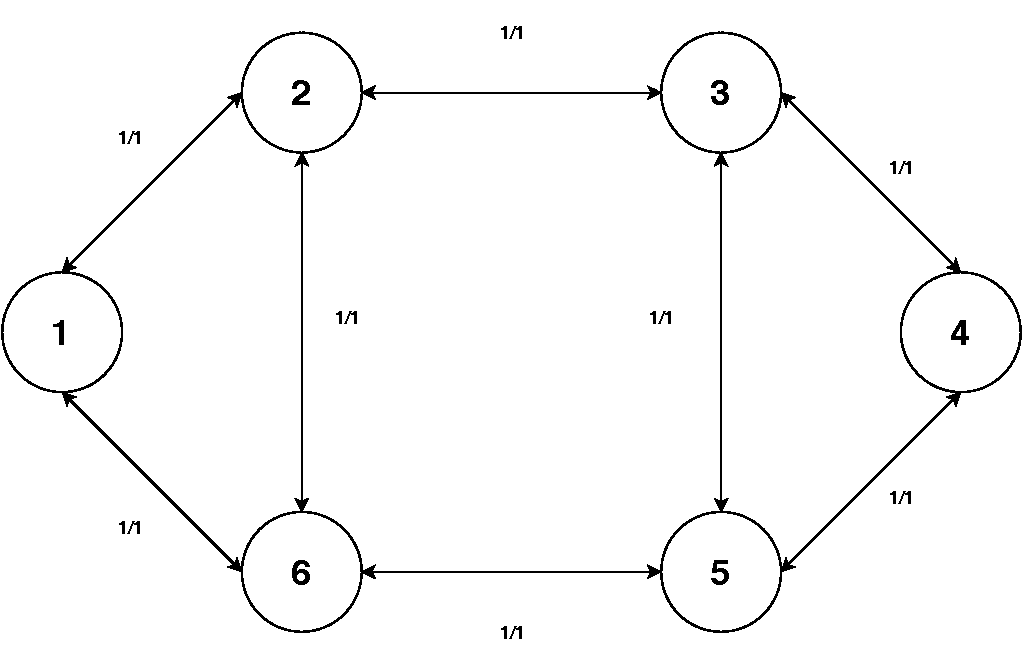
\includegraphics[width=0.55\textwidth]{fig/logos/lowPhysicalTopology.pdf}
    \caption{Physical topology after the dimensioning process for low scenario traffic.}
  \end{center}
  \label{lowPhysicalTopology}
\end{figure}

In a first instance the resulting physical topology of the reference network is presented above in figure \ref{lowPhysicalTopology} and the traffic model utilized for this specific scenario is referred in section \ref{low}. It becomes noticeable that all physical links are in use for this scenario.\\ \\

Below in table \ref{lowLinks} information regarding the global constitution of all network links is provided, the number of optical channels and the amplifiers present in each link is calculated through equations \ref{Capex_Link} and \ref{Capex_amplifiers}, respectively. 

\vspace{11pt}

\begin{table}[H]
\centering
\begin{tabular}{|c|c|c|}
\hline
\multicolumn{3}{|c|}{Information regarding links} \\ \hline
Bidirectional Link & Optical Channels & Amplifiers \\ \hline
Node 1 \textless{}-\textgreater Node 2 & 3 & 3 \\ \hline
Node 1 \textless{}-\textgreater Node 6 & 2 & 1 \\ \hline
Node 2 \textless{}-\textgreater Node 3 & 6 & 3 \\ \hline
Node 2 \textless{}-\textgreater Node 6 & 4 & 1 \\ \hline
Node 3 \textless{}-\textgreater Node 4 & 3 & 2 \\ \hline
Node 3 \textless{}-\textgreater Node 5 & 3 & 0 \\ \hline
Node 4 \textless{}-\textgreater Node 5 & 2 & 1 \\ \hline
Node 5 \textless{}-\textgreater Node 6 & 5 & 5 \\ \hline
\end{tabular}
\caption{Table with information regarding links for low traffic scenario.}
\label{lowLinks}
\end{table}

\vspace{11pt}

In table \ref{nodeLow} is presented detailed information regarding all the network nodes, the number of tributary ports is calculated through equation \ref{EXC_pexc1_transparent}, the number of add ports through \ref{OXC_poxc_transparent2} and the number of long-reach transponders through equation \ref{EXC_pexc2_transparent}.

\vspace{17pt}

\begin{table}[H]
\centering
\begin{tabular}{|c|c|c|c|c|c|}
\hline
\multicolumn{6}{|c|}{Information regarding nodes} \\ \hline
\multicolumn{2}{|c|}{} & \multicolumn{2}{c|}{Electrical part} & \multicolumn{2}{c|}{Optical part} \\ \hline
Node & Resulting Nodal Degree & Tributary Ports & LR Transponders & Add Ports & Line Ports \\ \hline
1 & 2 & 58 & 5 & 5 & 5 \\ \hline
2 & 3 & 46 & 7 & 7 & 13 \\ \hline
3 & 3 & 36 & 6 & 6 & 12 \\ \hline
4 & 2 & 40 & 5 & 5 & 5 \\ \hline
5 & 3 & 48 & 8 & 8 & 10 \\ \hline
6 & 3 & 44 & 9 & 9 & 11 \\ \hline
\end{tabular}
\caption{Table with information regarding nodes for low traffic scenario.}
\label{nodeLow}
\end{table}

\vspace{11pt}

Below, are presented some more tables properly identified that contain specific information regarding each of the nodes that comprise the reference network, after the dimensioning process. It becomes possible to analyze how many tributary ports each node contain and the respective bit-rates, the number of add and line ports connected and also the number of transponders used. In some cases the number of add ports and line ports in a node may differ, this happens if some of the traffic processed by the node is not originating from there, i.e. that node is not the source node for all the demands there processed. Having that said, when a node is equal to the source of a demand, it means that an add port and a line port are in use, otherwise, it means that through ports are used and in this case the number of ports is double the number of optical channels that go through the node.


\begin{table}[H]
\centering
\begin{tabular}{|c|c|c|}
\hline
\multicolumn{3}{|c|}{Detailed description of node 1} \\ \hline
Electrical part & Number of total demands & Bit rate \\ \hline
58 tributary ports & \begin{tabular}[c]{@{}c@{}}26\\ 26\\ 6\end{tabular} & \begin{tabular}[c]{@{}c@{}}ODU0\\ ODU1\\ ODU2\end{tabular} \\ \hline
 & Node \textless{}-Optical Channels-\textgreater Node & Bit rate \\ \hline
5 LR Transponders & \begin{tabular}[c]{@{}c@{}}1 \textless{}- 1 -\textgreater 2\\ 1 \textless{}- 1 -\textgreater 3\\ 1 \textless{}- 1 -\textgreater 4\\ 1 \textless{}- 1 -\textgreater 5\\ 1 \textless{}- 1 -\textgreater 6\end{tabular} & 100 Gbit/s \\ \hline
Optical part & Node \textless{}-Optical Channels-\textgreater Node & Bit rate \\ \hline
5 Add Ports & \begin{tabular}[c]{@{}c@{}}1 \textless{}- 1 -\textgreater 2\\ 1 \textless{}- 1 -\textgreater 3\\ 1 \textless{}- 1 -\textgreater 4\\ 1 \textless{}- 1 -\textgreater 5\\ 1 \textless{}- 1 -\textgreater 6\end{tabular} & \multirow{2}{*}{100 Gbit/s} \\ \cline{1-2}
5 Line Ports & \begin{tabular}[c]{@{}c@{}}1 \textless{}- 3 -\textgreater 2\\ 1 \textless{}- 2 -\textgreater 6\end{tabular} &  \\ \hline
\end{tabular}
\caption{Detailed description of node 1 for low traffic scenario.}
\end{table}


In this particular case, for node 1 the number of add ports and line ports is the same, which means that all the traffic processed by the node is originating from there.
\vspace{11pt}

\begin{table}[H]
\centering
\begin{tabular}{|c|c|c|}
\hline
\multicolumn{3}{|c|}{Detailed description of node 2} \\ \hline
Electrical part & Number of total demands & Bit rate \\ \hline
46 tributary ports & \begin{tabular}[c]{@{}c@{}}22\\ 14\\ 4\\ 4\\ 2\end{tabular} & \begin{tabular}[c]{@{}c@{}}ODU0\\ ODU1\\ ODU2\\ \\ ODU3\\ ODU4\end{tabular} \\ \hline
 & Node \textless{}-Optical Channels-\textgreater Node & Bit rate \\ \hline
7 LR Transponders & \begin{tabular}[c]{@{}c@{}}2 \textless{}- 1 -\textgreater 1\\ 2 \textless{}- 1 -\textgreater 3\\ 2 \textless{}- 1 -\textgreater 4\\ 2 \textless{}- 1 -\textgreater 5\\ 2 \textless{}- 3 -\textgreater 6\end{tabular} & 100 Gbit/s \\ \hline
Optical part & Node \textless{}-Optical Channels-\textgreater Node & Bit rate \\ \hline
7 Add Ports & \begin{tabular}[c]{@{}c@{}}2 \textless{}- 1 -\textgreater 1\\ 2 \textless{}- 1 -\textgreater 3\\ 2 \textless{}- 1 -\textgreater 4\\ 2 \textless{}- 1 -\textgreater 5\\ 2 \textless{}- 3 -\textgreater 6\end{tabular} & \multirow{2}{*}{100 Gbit/s} \\ \cline{1-2}
13 Line Ports & \begin{tabular}[c]{@{}c@{}}2 \textless{}- 3 -\textgreater 1\\ 2 \textless{}- 6 -\textgreater 3\\ \\ 2 \textless{}- 4 -\textgreater 6\end{tabular} &  \\ \hline
\end{tabular}
\caption{Detailed description of node 2 for low traffic scenario.}
\end{table}

\begin{table}[H]
\centering
\begin{tabular}{|c|c|c|}
\hline
\multicolumn{3}{|c|}{Detailed description of node 3} \\ \hline
Electrical part & Number of total demands & Bit rate \\ \hline
36 tributary ports & \begin{tabular}[c]{@{}c@{}}14\\ 12\\ 6\\ 4\end{tabular} & \begin{tabular}[c]{@{}c@{}}ODU0\\ ODU1\\ ODU2\\ ODU3\end{tabular} \\ \hline
 & Node \textless{}-Optical Channels-\textgreater Node & Bit rate \\ \hline
6 LR Transponders & \begin{tabular}[c]{@{}c@{}}3 \textless{}- 1 -\textgreater 1\\ 3 \textless{}- 1 -\textgreater 2\\ 3 \textless{}- 1 -\textgreater 4\\ 3 \textless{}- 2 -\textgreater 5\\ 3 \textless{}- 3 -\textgreater 6\end{tabular} & 100 Gbit/s \\ \hline
Optical part & Node \textless{}-Optical Channels-\textgreater Node & Bit rate \\ \hline
6 Add Ports & \begin{tabular}[c]{@{}c@{}}3 \textless{}- 1 -\textgreater 1\\ 3 \textless{}- 1 -\textgreater 2\\ 3 \textless{}- 1 -\textgreater 4\\ 3 \textless{}- 2 -\textgreater 5\\ 3 \textless{}- 3 -\textgreater 6\end{tabular} & \multirow{2}{*}{100 Gbit/s} \\ \cline{1-2}
12 Line Ports & \begin{tabular}[c]{@{}c@{}}3 \textless{}- 6 -\textgreater 2\\ 3 \textless{}- 3 -\textgreater 4\\ 3 \textless{}- 3 -\textgreater 5\end{tabular} &  \\ \hline
\end{tabular}
\caption{Detailed description of node 3 for low traffic scenario.}
\end{table}

\begin{table}[H]
\centering
\begin{tabular}{|c|c|c|}
\hline
\multicolumn{3}{|c|}{Detailed description of node 4} \\ \hline
Electrical part & Number of total demands & Bit rate \\ \hline
40 tributary ports & \begin{tabular}[c]{@{}c@{}}14\\ 20\\ 6\end{tabular} & \begin{tabular}[c]{@{}c@{}}ODU0\\ ODU1\\ ODU2\end{tabular} \\ \hline
 & Node \textless{}-Optical Channels-\textgreater Node & Bit rate \\ \hline
5 LR Transponders & \begin{tabular}[c]{@{}c@{}}4 \textless{}- 1 -\textgreater 1\\ 4 \textless{}- 1 -\textgreater 2\\ 4 \textless{}- 1 -\textgreater 3\\ 4 \textless{}- 2 -\textgreater 5\\ 4 \textless{}- 3 -\textgreater 6\end{tabular} & 100 Gbit/s \\ \hline
Optical part & Node \textless{}-Optical Channels-\textgreater Node & Bit rate \\ \hline
5 Add Ports & \begin{tabular}[c]{@{}c@{}}4 \textless{}- 1 -\textgreater 1\\ 4 \textless{}- 1 -\textgreater 2\\ 4 \textless{}- 1 -\textgreater 3\\ 4 \textless{}- 2 -\textgreater 5\\ 4 \textless{}- 3 -\textgreater 6\end{tabular} & \multirow{2}{*}{100 Gbit/s} \\ \cline{1-2}
5 Line Ports & \begin{tabular}[c]{@{}c@{}}4 \textless{}- 3 -\textgreater 3\\ 4 \textless{}- 2 -\textgreater 5\end{tabular} &  \\ \hline
\end{tabular}
\caption{Detailed description of node 4 for low traffic scenario.}
\end{table}

\begin{table}[H]
\centering
\begin{tabular}{|c|c|c|}
\hline
\multicolumn{3}{|c|}{Detailed description of node 5} \\ \hline
Electrical part & Number of total demands & Bit rate \\ \hline
48 tributary ports & \begin{tabular}[c]{@{}c@{}}28\\ 8\\ 8\\ 2\\ 2\end{tabular} & \begin{tabular}[c]{@{}c@{}}ODU0\\ ODU1\\ ODU2\\ \\ ODU3\\ ODU4\end{tabular} \\ \hline
 & Node \textless{}-Optical Channels-\textgreater Node & Bit rate \\ \hline
8 LR Transponders & \begin{tabular}[c]{@{}c@{}}5 \textless{}- 1 -\textgreater 1\\ 5 \textless{}- 1 -\textgreater 2\\ 5 \textless{}- 2 -\textgreater 3\\ 5 \textless{}- 1 -\textgreater 4\\ 5 \textless{}- 3 -\textgreater 6\end{tabular} & 100 Gbit/s \\ \hline
Optical part & Node \textless{}-Optical Channels-\textgreater Node & Bit rate \\ \hline
8 Add Ports & \begin{tabular}[c]{@{}c@{}}5 \textless{}- 1 -\textgreater 1\\ 5 \textless{}- 1 -\textgreater 2\\ 5 \textless{}- 2 -\textgreater 3\\ 5 \textless{}- 1 -\textgreater 4\\ 5 \textless{}- 3 -\textgreater 6\end{tabular} & \multirow{2}{*}{100 Gbit/s} \\ \cline{1-2}
10 Line Ports & \begin{tabular}[c]{@{}c@{}}5 \textless{}- 3 -\textgreater 3\\ 5 \textless{}- 2 -\textgreater 4\\ \\ 5 \textless{}- 5 -\textgreater 6\end{tabular} &  \\ \hline
\end{tabular}
\caption{Detailed description of node 5 for low traffic scenario.}
\end{table}

\begin{table}[H]
\centering
\begin{tabular}{|c|c|c|}
\hline
\multicolumn{3}{|c|}{Detailed description of node 6} \\ \hline
Electrical part & Number of total demands & Bit rate \\ \hline
44 tributary ports & \begin{tabular}[c]{@{}c@{}}16\\ 20\\ 2\\ 2\\ 4\end{tabular} & \begin{tabular}[c]{@{}c@{}}ODU0\\ ODU1\\ ODU2\\ ODU3\\ ODU4\end{tabular} \\ \hline
 & Node \textless{}-Optical Channels-\textgreater Node & Bit rate \\ \hline
9 LR Transponders & \begin{tabular}[c]{@{}c@{}}6 \textless{}- 1 -\textgreater 1\\ 6 \textless{}- 3 -\textgreater 2\\ 6 \textless{}- 1 -\textgreater 3\\ 6 \textless{}- 1 -\textgreater 4\\ 6 \textless{}- 3 -\textgreater 5\end{tabular} & 100 Gbit/s \\ \hline
Optical part & Node \textless{}-Optical Channels-\textgreater Node & Bit rate \\ \hline
9 Add Ports & \begin{tabular}[c]{@{}c@{}}6 \textless{}- 1 -\textgreater 1\\ 6 \textless{}- 3 -\textgreater 2\\ 6 \textless{}- 1 -\textgreater 3\\ 6 \textless{}- 1 -\textgreater 4\\ 6 \textless{}- 3 -\textgreater 5\end{tabular} & \multirow{2}{*}{100 Gbit/s} \\ \cline{1-2}
11 Line Ports & \begin{tabular}[c]{@{}c@{}}6 \textless{}- 2 -\textgreater 1\\ 6 \textless{}- 4 -\textgreater 2\\ 6 \textless{}- 5 -\textgreater 5\end{tabular} &  \\ \hline
\end{tabular}
\caption{Detailed description of node 6 for low traffic scenario.}
\end{table}
\clearpage
In the following table \ref{routingscheme1}, the routing information is in focus. Again, the paths are considered bidirectional and as such the paths between the same pair of nodes but in opposite directions are still the same.  

\begin{table}[H]
\centering
\scalebox{0.84}{
\begin{tabular}{|c|c|c|c|c|c|c|c|}
\hline
\multicolumn{8}{|c|}{Routing Scheme} \\ \hline
Source & Destination & Links & ODU0 & ODU1 & ODU2 & ODU3 & ODU4 \\ \hline
1 & 2 & \{(1,2)\} & 10 & 4 & 2 & 0 & 0 \\ \hline
1 & 3 & \{(1,2),(2,3)\} & 2 & 8 & 2 & 0 & 0 \\ \hline
1 & 4 & \{(1,2),(2,3),(3,4)\} & 6 & 4 & 2 & 0 & 0 \\ \hline
1 & 5 & \{(1,6),(6,5)\} & 2 & 0 & 0 & 0 & 0 \\ \hline
1 & 6 & \{(1,6)\} & 6 & 10 & 0 & 0 & 0 \\ \hline
2 & 3 & \{(2,3)\} & 0 & 0 & 0 & 2 & 0 \\ \hline
2 & 4 & \{(2,3),(3,4)\} & 2 & 6 & 0 & 0 & 0 \\ \hline
2 & 5 & \{(2,3),(3,5)\} & 10 & 2 & 2 & 0 & 0 \\ \hline
2 & 6 & \{(2,6)\} & 0 & 2 & 0 & 2 & 2 \\ \hline
3 & 4 & \{(3,4)\} & 2 & 2 & 2 & 0 & 0 \\ \hline
3 & 5 & \{(3,5)\} & 8 & 2 & 2 & 2 & 0 \\ \hline
3 & 6 & \{(3,2),(2,6)\} & 2 & 0 & 0 & 0 & 0 \\ \hline
4 & 5 & \{(4,5)\} & 2 & 2 & 2 & 0 & 0 \\ \hline
4 & 6 & \{(4,5),(5,6)\} & 2 & 6 & 0 & 0 & 0 \\ \hline
5 & 6 & \{(5,6)\} & 6 & 2 & 2 & 0 & 2 \\ \hline
\end{tabular}}
\caption{Detailed description of the routing process for low traffic scenario.}
\label{routingscheme1}
\end{table}

Finally, in table \ref{capexresults1} is presented the final CAPEX results obtained for the low traffic scenario, obtained through the heuristic model.

\begin{table}[H]
\centering
\scalebox{0.9}{
\begin{tabular}{|c|c|c|c|c|c|c|}
\hline
\multicolumn{7}{|c|}{Network CAPEX} \\ \hline
\multicolumn{3}{|c|}{} & Quantity & Unit Price & Cost & Total \\ \hline
\multirow{3}{*}{\begin{tabular}[c]{@{}c@{}}Link\\ Cost\end{tabular}} & \multicolumn{2}{c|}{OLTs} & 16 & 15 000 \euro & 240 000 \euro & \multirow{3}{*}{584 000 \euro} \\ \cline{2-6}
 & \multicolumn{2}{c|}{Optical Channels} & 56 & 5000 \euro & 280 000 \euro &  \\ \cline{2-6}
 & \multicolumn{2}{c|}{Amplifiers} & 32 & 2000 \euro & 64 000 \euro &  \\ \hline
\multirow{10}{*}{\begin{tabular}[c]{@{}c@{}}Node\\ Cost\end{tabular}} & \multirow{7}{*}{Electrical} & EXCs & 6 & 10 000 \euro & 60 000 \euro & \multirow{10}{*}{1 020 000 \euro} \\ \cline{3-6}
 &  & ODU0 Ports & 120 & 100 \euro/Gbit/s & 15 000 \euro &  \\ \cline{3-6}
 &  & ODU1 Ports & 100 & 100 \euro/Gbit/s & 25 000 \euro &  \\ \cline{3-6}
 &  & ODU2 Ports & 32 & 100 \euro/Gbit/s & 32 000 \euro &  \\ \cline{3-6}
 &  & ODU3 Ports & 12 & 100 \euro/Gbit/s & 48 000 \euro &  \\ \cline{3-6}
 &  & ODU4 Ports & 8 & 100 \euro/Gbit/s & 80 000 \euro &  \\ \cline{3-6}
 &  & LR Transponders & 40 & 100 \euro/Gbit/s & 400 000 \euro &  \\ \cline{2-6}
 & \multirow{3}{*}{Optical} & OXCs & 6 & 20 000 \euro & 120 000 \euro &  \\ \cline{3-6}
 &  & \multirow{2}{*}{OXC Ports} & \multirow{2}{*}{96} & \multirow{2}{*}{2 500 \euro} & \multirow{2}{*}{240 000 \euro} &  \\
 &  &  &  &  &  &  \\ \hline
\multicolumn{6}{|c|}{Total Network Cost} & 1 604 000 \euro \\ \hline
\end{tabular}}
\caption{Detailed description of CAPEX for low traffic scenario.}
\label{capexresults1}
\end{table}

\subsubsection{Medium traffic}

In a first instance the resulting physical topology of the reference network is presented below in figure \ref{mediumPhysicalTopology}. The traffic model utilized for this specific scenario is referred in section \ref{medium}.

\begin{figure}[H]
  \begin{center}
    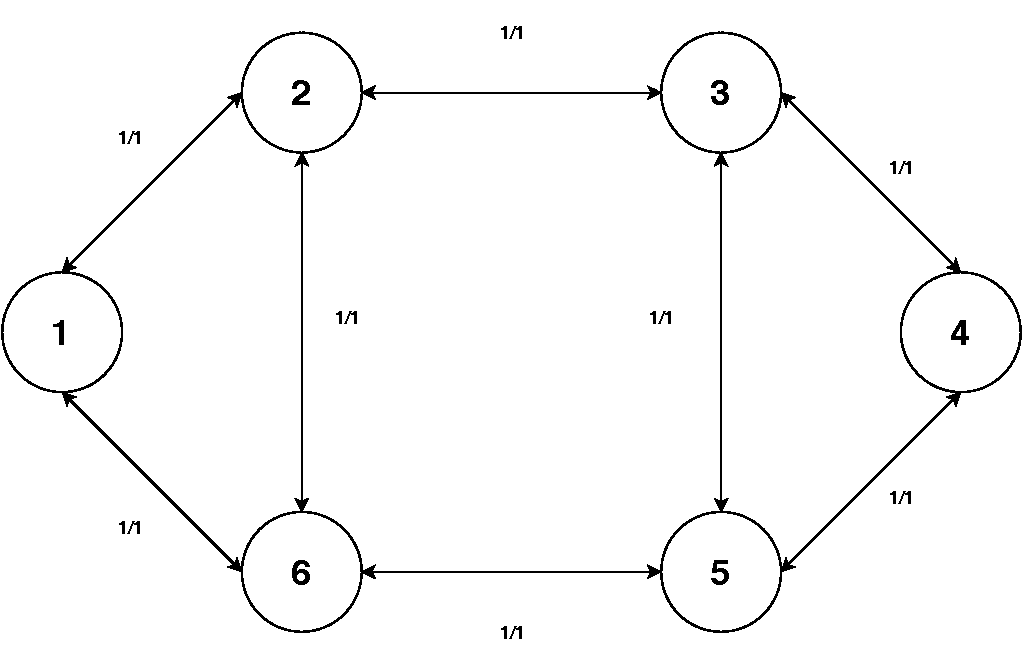
\includegraphics[width=0.6\textwidth]{fig/logos/lowPhysicalTopology.pdf}
    \caption{Physical topology after dimensioning for medium scenario traffic.}
  \end{center}
  \label{mediumPhysicalTopology}
\end{figure}

It is noticeable that all physical links are in use for this scenario. Below in table \ref{mediumLinks} information regarding the global constitution of all network links is provided, the number of optical channels and the amplifiers present in each link is calculated through equations \ref{Capex_Link} and \ref{Capex_amplifiers}, respectively.


\begin{table}[H]
\centering
\begin{tabular}{|c|c|c|}
\hline
\multicolumn{3}{|c|}{Information regarding links} \\ \hline
Bidirectional Link & Optical Channels & Amplifiers \\ \hline
Node 1 \textless{}-\textgreater Node 2 & 8 & 3 \\ \hline
Node 1 \textless{}-\textgreater Node 6 & 3 & 1 \\ \hline
Node 2 \textless{}-\textgreater Node 3 & 14 & 3 \\ \hline
Node 2 \textless{}-\textgreater Node 6 & 16 & 1 \\ \hline
Node 3 \textless{}-\textgreater Node 4 & 5 & 2 \\ \hline
Node 3 \textless{}-\textgreater Node 5 & 8 & 0 \\ \hline
Node 4 \textless{}-\textgreater Node 5 & 3 & 1 \\ \hline
Node 5 \textless{}-\textgreater Node 6 & 14 & 5 \\ \hline
\end{tabular}
\caption{Links information for medium traffic scenario.}
\label{mediumLinks}
\end{table}


In table \ref{nodeMedium} is presented detailed information regarding all the network nodes, the number of tributary ports is calculated through equation \ref{EXC_pexc1_transparent}, the number of add ports through \ref{OXC_poxc_transparent2} and the number of long-reach transponders through equation \ref{EXC_pexc2_transparent}.

\vspace{17pt}

\begin{table}[H]
\centering
\scalebox{0.9}{
\begin{tabular}{|c|c|c|c|c|c|}
\hline
\multicolumn{6}{|c|}{Information regarding nodes} \\ \hline
\multicolumn{2}{|c|}{} & \multicolumn{2}{c|}{Electrical part} & \multicolumn{2}{c|}{Optical part} \\ \hline
Node & Resulting Nodal Degree & Tributary Ports & LR Transponders & Add Ports & Line Ports \\ \hline
1 & 2 & 290 & 11 & 11 & 11 \\ \hline
2 & 3 & 230 & 26 & 26 & 38 \\ \hline
3 & 3 & 180 & 17 & 17 & 27 \\ \hline
4 & 2 & 200 & 8 & 8 & 8 \\ \hline
5 & 3 & 240 & 23 & 23 & 25 \\ \hline
6 & 3 & 220 & 31 & 31 & 33 \\ \hline
\end{tabular}}
\caption{Node information for medium traffic scenario.}
\label{nodeMedium}
\end{table}

\vspace{11pt}

Below, are presented some more tables properly identified that contain specific information regarding each of the nodes that comprise the reference network, after the dimensioning process. %It becomes possible to analyze how many tributary ports each node contain and the respective bit-rates, the number of optical channels connecting to the node, and also, regarding the optical part of the nodes, the number of add and line ports connected. %In some cases the number of add ports and line ports in a node may differ, this happens if some of the traffic processed by the node is not originating from there, i.e. that node is not the source node for all the demands there processed. Having that said, when a node is equal to the source of a demand, it means that an add port and a line port are in use, otherwise, it means that through ports are used and in this case the number of ports is double the number of optical channels that go through the node.


\begin{table}[H]
\centering
\scalebox{0.95}{
\begin{tabular}{|c|c|c|}
\hline
\multicolumn{3}{|c|}{Detailed description of node 1} \\ \hline
Electrical part & Number of total demands & Bit rate \\ \hline
290 tributary ports & \begin{tabular}[c]{@{}c@{}}130\\ 130\\ 30\end{tabular} & \begin{tabular}[c]{@{}c@{}}ODU0\\ ODU1\\ ODU2\end{tabular} \\ \hline
 & Node \textless{}-Optical Channels-\textgreater Node & Bit rate \\ \hline
11 LR Transponders & \begin{tabular}[c]{@{}c@{}}1 \textless{}- 3 -\textgreater 2\\ 1 \textless{}- 3 -\textgreater 3\\ 1 \textless{}- 2 -\textgreater 4\\ 1 \textless{}- 1 -\textgreater 5\\ 1 \textless{}- 2 -\textgreater 6\end{tabular} & 100 Gbit/s \\ \hline
Optical part & Node \textless{}-Optical Channels-\textgreater Node & Bit rate \\ \hline
11 Add Ports & \begin{tabular}[c]{@{}c@{}}1 \textless{}- 3 -\textgreater 2\\ 1 \textless{}- 3 -\textgreater 3\\ 1 \textless{}- 2 -\textgreater 4\\ 1 \textless{}- 1 -\textgreater 5\\ 1 \textless{}- 2 -\textgreater 6\end{tabular} & \multirow{2}{*}{100 Gbit/s} \\ \cline{1-2}
11 Line Ports & \begin{tabular}[c]{@{}c@{}}1 \textless{}- 8 -\textgreater 2\\ 1 \textless{}- 3 -\textgreater 6\end{tabular} &  \\ \hline
\end{tabular}}
\caption{Detailed description of node 1 for medium traffic scenario.}
\end{table}


\vspace{11pt}

\begin{table}[H]
\centering
\begin{tabular}{|c|c|c|}
\hline
\multicolumn{3}{|c|}{Detailed description of node 2} \\ \hline
Electrical part & Number of total demands & Bit rate \\ \hline
230 tributary ports & \begin{tabular}[c]{@{}c@{}}110\\ 70\\ 20\\ 20\\ 10\end{tabular} & \begin{tabular}[c]{@{}c@{}}ODU0\\ ODU1\\ ODU2\\ ODU3\\ ODU4\end{tabular} \\ \hline
 & Node \textless{}-Optical Channels-\textgreater Node & Bit rate \\ \hline
26 LR Transponders & \begin{tabular}[c]{@{}c@{}}2 \textless{}- 3 -\textgreater 1\\ 2 \textless{}- 5 -\textgreater 3\\ 2 \textless{}- 1 -\textgreater 4\\ 2 \textless{}- 2 -\textgreater 5\\ 2 \textless{}- 15 -\textgreater 6\end{tabular} & 100 Gbit/s \\ \hline
Optical part & Node \textless{}-Optical Channels-\textgreater Node & Bit rate \\ \hline
26 Add Ports & \begin{tabular}[c]{@{}c@{}}2 \textless{}- 3 -\textgreater 1\\ 2 \textless{}- 5 -\textgreater 3\\ 2 \textless{}- 1 -\textgreater 4\\ 2 \textless{}- 2 -\textgreater 5\\ 2 \textless{}- 15 -\textgreater 6\end{tabular} & \multirow{2}{*}{100 Gbit/s} \\ \cline{1-2}
38 Line Ports & \begin{tabular}[c]{@{}c@{}}2 \textless{}- 8 -\textgreater 1\\ 2 \textless{}- 14 -\textgreater 3\\ 2 \textless{}- 16 -\textgreater 6\end{tabular} &  \\ \hline
\end{tabular}
\caption{Detailed description of node 2 for medium traffic scenario.}
\end{table}

\begin{table}[H]
\centering
\begin{tabular}{|c|c|c|}
\hline
\multicolumn{3}{|c|}{Detailed description of node 3} \\ \hline
Electrical part & Number of total demands & Bit rate \\ \hline
180 tributary ports & \begin{tabular}[c]{@{}c@{}}70\\ 60\\ 30\\ 20\end{tabular} & \begin{tabular}[c]{@{}c@{}}ODU0\\ ODU1\\ ODU2\\ ODU3\end{tabular} \\ \hline
 & Node \textless{}-Optical Channels-\textgreater Node & Bit rate \\ \hline
17 LR Transponders & \begin{tabular}[c]{@{}c@{}}3 \textless{}- 3 -\textgreater 1\\ 3 \textless{}- 5 -\textgreater 2\\ 3 \textless{}- 2 -\textgreater 4\\ 3 \textless{}- 6 -\textgreater 5\\ 3 \textless{}- 1 -\textgreater 6\end{tabular} & 100 Gbit/s \\ \hline
Optical part & Node \textless{}-Optical Channels-\textgreater Node & Bit rate \\ \hline
17 Add Ports & \begin{tabular}[c]{@{}c@{}}3 \textless{}- 3 -\textgreater 1\\ 3 \textless{}- 5 -\textgreater 2\\ 3 \textless{}- 2 -\textgreater 4\\ 3 \textless{}- 6 -\textgreater 5\\ 3 \textless{}- 1 -\textgreater 6\end{tabular} & \multirow{2}{*}{100 Gbit/s} \\ \cline{1-2}
27 Line Ports & \begin{tabular}[c]{@{}c@{}}3 \textless{}- 14 -\textgreater 2\\ 3 \textless{}- 5 -\textgreater 4\\ 3 \textless{}- 8 -\textgreater 5\end{tabular} &  \\ \hline
\end{tabular}
\caption{Detailed description of node 3 for medium traffic scenario.}
\end{table}

\begin{table}[H]
\centering
\begin{tabular}{|c|c|c|}
\hline
\multicolumn{3}{|c|}{Detailed description of node 4} \\ \hline
Electrical part & Number of total demands & Bit rate \\ \hline
200 tributary ports & \begin{tabular}[c]{@{}c@{}}70\\ 100\\ 30\end{tabular} & \begin{tabular}[c]{@{}c@{}}ODU0\\ ODU1\\ ODU2\end{tabular} \\ \hline
 & Node \textless{}-Optical Channels-\textgreater Node & Bit rate \\ \hline
8 LR Transponders & \begin{tabular}[c]{@{}c@{}}4 \textless{}- 2 -\textgreater 1\\ 4 \textless{}- 1 -\textgreater 2\\ 4 \textless{}- 2 -\textgreater 3\\ 4 \textless{}- 2 -\textgreater 5\\ 4 \textless{}- 1 -\textgreater 6\end{tabular} & 100 Gbit/s \\ \hline
Optical part & Node \textless{}-Optical Channels-\textgreater Node & Bit rate \\ \hline
8 Add Ports & \begin{tabular}[c]{@{}c@{}}4 \textless{}- 2 -\textgreater 1\\ 4 \textless{}- 1 -\textgreater 2\\ 4 \textless{}- 2 -\textgreater 3\\ 4 \textless{}- 2 -\textgreater 5\\ 4 \textless{}- 1 -\textgreater 6\end{tabular} & \multirow{2}{*}{100 Gbit/s} \\ \cline{1-2}
8 Line Ports & \begin{tabular}[c]{@{}c@{}}4 \textless{}- 5 -\textgreater 3\\ 4 \textless{}- 3 -\textgreater 5\end{tabular} &  \\ \hline
\end{tabular}
\caption{Detailed description of node 4 for medium traffic scenario.}
\end{table}

\begin{table}[H]
\centering
\begin{tabular}{|c|c|c|}
\hline
\multicolumn{3}{|c|}{Detailed description of node 5} \\ \hline
Electrical part & Number of total demands & Bit rate \\ \hline
240 tributary ports & \begin{tabular}[c]{@{}c@{}}140\\ 40\\ 40\\ 10\\ 10\end{tabular} & \begin{tabular}[c]{@{}c@{}}ODU0\\ ODU1\\ ODU2\\ ODU3\\ ODU4\end{tabular} \\ \hline
 & Node \textless{}-Optical Channels-\textgreater Node & Bit rate \\ \hline
23 LR Transponders & \begin{tabular}[c]{@{}c@{}}5 \textless{}- 1 -\textgreater 1\\ 5 \textless{}- 2 -\textgreater 2\\ 5 \textless{}- 6 -\textgreater 3\\ 5 \textless{}- 2 -\textgreater 4\\ 5 \textless{}- 12 -\textgreater 6\end{tabular} & 100 Gbit/s \\ \hline
Optical part & Node \textless{}-Optical Channels-\textgreater Node & Bit rate \\ \hline
23 Add Ports & \begin{tabular}[c]{@{}c@{}}5 \textless{}- 1 -\textgreater 1\\ 5 \textless{}- 2 -\textgreater 2\\ 5 \textless{}- 6 -\textgreater 3\\ 5 \textless{}- 2 -\textgreater 4\\ 5 \textless{}- 12 -\textgreater 6\end{tabular} & \multirow{2}{*}{100 Gbit/s} \\ \cline{1-2}
25 Line Ports & \begin{tabular}[c]{@{}c@{}}5 \textless{}- 8 -\textgreater 3\\ 5 \textless{}- 3 -\textgreater 4\\ 5 \textless{}- 14 -\textgreater 6\end{tabular} &  \\ \hline
\end{tabular}
\caption{Detailed description of node 5 for medium traffic scenario.}
\end{table}

\begin{table}[H]
\centering
\begin{tabular}{|c|c|c|}
\hline
\multicolumn{3}{|c|}{Detailed description of node 6} \\ \hline
Electrical part & Number of total demands & Bit rate \\ \hline
220 tributary ports & \begin{tabular}[c]{@{}c@{}}80\\ 100\\ 10\\ 10\\ 20\end{tabular} & \begin{tabular}[c]{@{}c@{}}ODU0\\ ODU1\\ ODU2\\ ODU3\\ ODU4\end{tabular} \\ \hline
 & Node \textless{}-Optical Channels-\textgreater Node & Bit rate \\ \hline
31 LR Transponders & \begin{tabular}[c]{@{}c@{}}6 \textless{}- 2 -\textgreater 1\\ 6 \textless{}- 15 -\textgreater 2\\ 6 \textless{}- 1 -\textgreater 3\\ 6 \textless{}- 1 -\textgreater 4\\ 6 \textless{}- 12 -\textgreater 5\end{tabular} & 100 Gbit/s \\ \hline
Optical part & Node \textless{}-Optical Channels-\textgreater Node & Bit rate \\ \hline
31 Add Ports & \begin{tabular}[c]{@{}c@{}}6 \textless{}- 2 -\textgreater 1\\ 6 \textless{}- 15 -\textgreater 2\\ 6 \textless{}- 1 -\textgreater 3\\ 6 \textless{}- 1 -\textgreater 4\\ 6 \textless{}- 12 -\textgreater 5\end{tabular} & \multirow{2}{*}{100 Gbit/s} \\ \cline{1-2}
33 Line Ports & \begin{tabular}[c]{@{}c@{}}6 \textless{}- 3 -\textgreater 1\\ 6 \textless{}- 16 -\textgreater 2\\ 6 \textless{}- 14 -\textgreater 5\end{tabular} &  \\ \hline
\end{tabular}
\caption{Detailed description of node 6 for medium traffic scenario.}
\end{table}
\clearpage
In the following table \ref{routingscheme1}, the routing information is in focus. %Again, the paths are considered bidirectional and as such the paths between the same pair of nodes but in opposite directions are still the same.  

\begin{table}[H]
\centering
\scalebox{0.9}{
\begin{tabular}{|c|c|c|c|c|c|c|c|}
\hline
\multicolumn{8}{|c|}{Routing Scheme} \\ \hline
Source & Destination & Links & ODU0 & ODU1 & ODU2 & ODU3 & ODU4 \\ \hline
1 & 2 & \{(1,2)\} & 50 & 20 & 10 & 0 & 0 \\ \hline
1 & 3 & \{(1,2),(2,3)\} & 10 & 40 & 10 & 0 & 0 \\ \hline
1 & 4 & \{(1,2),(2,3),(3,4)\} & 30 & 20 & 10 & 0 & 0 \\ \hline
1 & 5 & \{(1,6),(6,5)\} & 10 & 0 & 0 & 0 & 0 \\ \hline
1 & 6 & \{(1,6)\} & 30 & 50 & 0 & 0 & 0 \\ \hline
2 & 3 & \{(2,3)\} & 0 & 0 & 0 & 10 & 0 \\ \hline
2 & 4 & \{(2,3),(3,4)\} & 10 & 30 & 0 & 0 & 0 \\ \hline
2 & 5 & \{(2,3),(3,5)\} & 50 & 10 & 10 & 0 & 0 \\ \hline
2 & 6 & \{(2,6)\} & 0 & 10 & 0 & 10 & 10 \\ \hline
3 & 4 & \{(3,4)\} & 10 & 10 & 10 & 0 & 0 \\ \hline
3 & 5 & \{(3,5)\} & 40 & 10 & 10 & 10 & 0 \\ \hline
3 & 6 & \{(3,2),(2,6)\} & 10 & 0 & 0 & 0 & 0 \\ \hline
4 & 5 & \{(4,5)\} & 10 & 10 & 10 & 0 & 0 \\ \hline
4 & 6 & \{(4,5),(5,6)\} & 10 & 30 & 0 & 0 & 0 \\ \hline
5 & 6 & \{(5,6)\} & 30 & 10 & 10 & 0 & 10 \\ \hline
\end{tabular}}
\caption{Detailed description of the routing process for medium traffic scenario.}
\end{table}

Finally, in table \ref{capexresults1} is presented the final CAPEX results obtained for the low traffic scenario, obtained through the heuristic model.

\begin{table}[H]
\centering
\scalebox{0.9}{
\begin{tabular}{|c|c|c|c|c|c|c|}
\hline
\multicolumn{7}{|c|}{Network CAPEX} \\ \hline
\multicolumn{3}{|c|}{} & Quantity & Unit Price & Cost & Total \\ \hline
\multirow{3}{*}{\begin{tabular}[c]{@{}c@{}}Link\\ Cost\end{tabular}} & \multicolumn{2}{c|}{OLTs} & 16 & 15 000 \euro & 240 000 \euro & \multirow{3}{*}{1 014 000 \euro} \\ \cline{2-6}
 & \multicolumn{2}{c|}{Optical Channels} & 142 & 5000 \euro & 710 000 \euro &  \\ \cline{2-6}
 & \multicolumn{2}{c|}{Amplifiers} & 32 & 2000 \euro & 64 000 \euro &  \\ \hline
\multirow{10}{*}{\begin{tabular}[c]{@{}c@{}}Node\\ Cost\end{tabular}} & \multirow{7}{*}{Electrical} & EXCs & 6 & 10 000 \euro & 60 000 \euro & \multirow{10}{*}{2 985 000 \euro} \\ \cline{3-6}
 &  & ODU0 Ports & 600 & 100 \euro/Gbit/s & 75 000 \euro &  \\ \cline{3-6}
 &  & ODU1 Ports & 500 & 100 \euro/Gbit/s & 125 000 \euro &  \\ \cline{3-6}
 &  & ODU2 Ports & 160 & 100 \euro/Gbit/s & 160 000 \euro &  \\ \cline{3-6}
 &  & ODU3 Ports & 60 & 100 \euro/Gbit/s & 240 000 \euro &  \\ \cline{3-6}
 &  & ODU4 Ports & 40 & 100 \euro/Gbit/s & 400 000 \euro &  \\ \cline{3-6}
 &  & LR Transponders & 116 & 100 \euro/Gbit/s & 1 160 000 \euro &  \\ \cline{2-6}
 & \multirow{3}{*}{Optical} & OXCs & 6 & 20 000 \euro & 120 000 \euro &  \\ \cline{3-6}
 &  & \multirow{2}{*}{OXC Ports} & \multirow{2}{*}{258} & \multirow{2}{*}{2 500 \euro} & \multirow{2}{*}{645 000 \euro} &  \\
 &  &  &  &  &  &  \\ \hline
\multicolumn{6}{|c|}{Total Network Cost} & 3 999 000 \euro \\ \hline
\end{tabular}}
\caption{Detailed description of CAPEX for medium traffic scenario.}
\end{table}
\subsubsection{High traffic}

In a first instance the resulting physical topology of the reference network is presented below in figure \ref{highPhysicalTopology}. The traffic model utilized for this specific scenario is mentioned in the section \ref{high}.

\begin{figure}[H]
  \begin{center}
    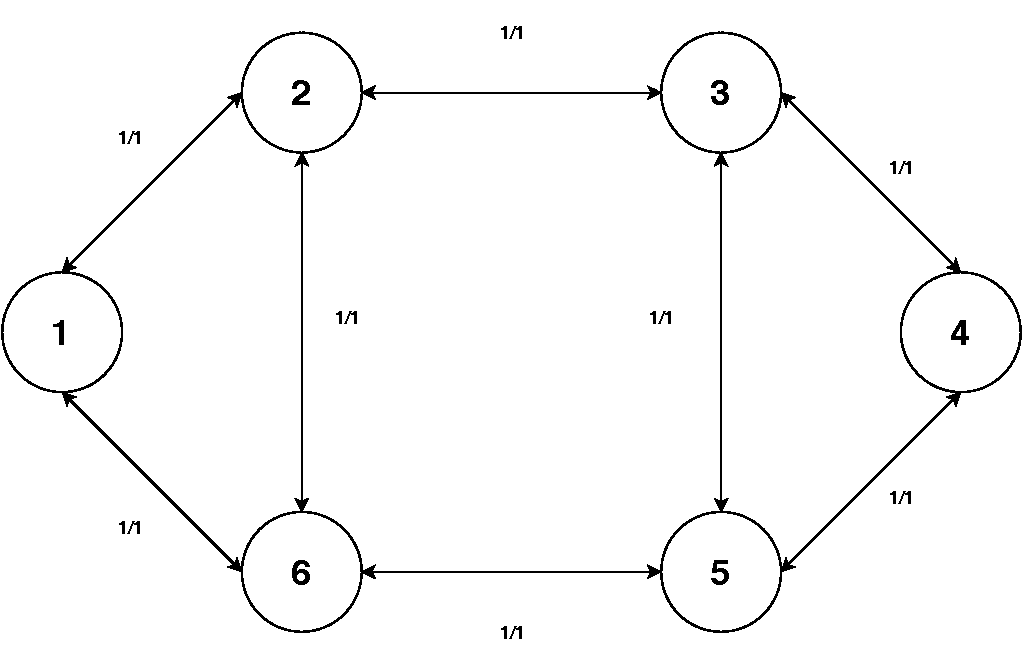
\includegraphics[width=0.6\textwidth]{fig/logos/lowPhysicalTopology.pdf}
    \caption{Physical topology after dimensioning process for high scenario traffic.}
  \end{center}
  \label{highPhysicalTopology}
\end{figure}

It is noticeable that all physical links are in use for this scenario. Below in table \ref{highLinks} information regarding the global constitution of all network links is provided, the number of optical channels and the amplifiers present in each link is calculated through equations \ref{Capex_Link} and \ref{Capex_amplifiers}, respectively.


\begin{table}[H]
\centering
\begin{tabular}{|c|c|c|}
\hline
\multicolumn{3}{|c|}{Information regarding links} \\ \hline
Bidirectional Link & Optical Channels & Amplifiers \\ \hline
Node 1 \textless{}-\textgreater Node 2 & 14 & 3 \\ \hline
Node 1 \textless{}-\textgreater Node 6 & 5 & 1 \\ \hline
Node 2 \textless{}-\textgreater Node 3 & 26 & 3 \\ \hline
Node 2 \textless{}-\textgreater Node 6 & 31 & 1 \\ \hline
Node 3 \textless{}-\textgreater Node 4 & 9 & 2 \\ \hline
Node 3 \textless{}-\textgreater Node 5 & 16 & 0 \\ \hline
Node 4 \textless{}-\textgreater Node 5 & 5 & 1 \\ \hline
Node 5 \textless{}-\textgreater Node 6 & 27 & 5 \\ \hline
\end{tabular}
\caption{Links information for high traffic scenario.}
\label{highLinks}
\end{table}



In table \ref{nodeHigh} is presented detailed information regarding all the network nodes, the number of tributary ports is calculated through equation \ref{EXC_pexc1_transparent}, the number of add ports through \ref{OXC_poxc_transparent2} and the number of long-reach transponders through equation \ref{EXC_pexc2_transparent}.



\begin{table}[H]
\centering
\scalebox{0.9}{
\begin{tabular}{|c|c|c|c|c|c|}
\hline
\multicolumn{6}{|c|}{Information regarding nodes} \\ \hline
\multicolumn{2}{|c|}{} & \multicolumn{2}{c|}{Electrical part} & \multicolumn{2}{c|}{Optical part} \\ \hline
Node & Resulting Nodal Degree & Tributary Ports & LR Transponders & Add Ports & Line Ports \\ \hline
1 & 2 & 580 & 19 & 19 & 19 \\ \hline
2 & 3 & 460 & 51 & 51 & 71 \\ \hline
3 & 3 & 360 & 31 & 31 & 51 \\ \hline
4 & 2 & 400 & 14 & 14 & 14 \\ \hline
5 & 3 & 480 & 44 & 44 & 48 \\ \hline
6 & 3 & 440 & 61 & 61 & 63 \\ \hline
\end{tabular}}
\caption{Node information for high traffic scenario.}
\label{nodeHigh}
\end{table}

\vspace{11pt}

Below, are presented some more tables properly identified that contain specific information regarding each of the nodes that comprise the reference network, after the dimensioning process.


\begin{table}[H]
\centering
\scalebox{1}{
\begin{tabular}{|c|c|c|}
\hline
\multicolumn{3}{|c|}{Detailed description of node 1} \\ \hline
Electrical part & Number of total demands & Bit rate \\ \hline
580 tributary ports & \begin{tabular}[c]{@{}c@{}}260\\ 260\\ 60\end{tabular} & \begin{tabular}[c]{@{}c@{}}ODU0\\ ODU1\\ ODU2\end{tabular} \\ \hline
 & Node \textless{}-Optical Channels-\textgreater Node & Bit rate \\ \hline
19 LR Transponders & \begin{tabular}[c]{@{}c@{}}1 \textless{}- 5 -\textgreater 2\\ 1 \textless{}- 5 -\textgreater 3\\ 1 \textless{}- 4 -\textgreater 4\\ 1 \textless{}- 1 -\textgreater 5\\ 1 \textless{}- 4 -\textgreater 6\end{tabular} & 100 Gbit/s \\ \hline
Optical part & Node \textless{}-Optical Channels-\textgreater Node & Bit rate \\ \hline
19 Add Ports & \begin{tabular}[c]{@{}c@{}}1 \textless{}- 5 -\textgreater 2\\ 1 \textless{}- 5 -\textgreater 3\\ 1 \textless{}- 4 -\textgreater 4\\ 1 \textless{}- 1 -\textgreater 5\\ 1 \textless{}- 4 -\textgreater 6\end{tabular} & \multirow{2}{*}{100 Gbit/s} \\ \cline{1-2}
19 Line Ports & \begin{tabular}[c]{@{}c@{}}1 \textless{}- 14 -\textgreater 2\\ 1 \textless{}- 5 -\textgreater 6\end{tabular} &  \\ \hline
\end{tabular}}
\caption{Detailed description of node 1 for high traffic scenario.}
\end{table}



\begin{table}[H]
\centering
\begin{tabular}{|c|c|c|}
\hline
\multicolumn{3}{|c|}{Detailed description of node 2} \\ \hline
Electrical part & Number of total demands & Bit rate \\ \hline
460 tributary ports & \begin{tabular}[c]{@{}c@{}}220\\ 140\\ 40\\ 40\\ 20\end{tabular} & \begin{tabular}[c]{@{}c@{}}ODU0\\ ODU1\\ ODU2\\ ODU3\\ ODU4\end{tabular} \\ \hline
 & Node \textless{}-Optical Channels-\textgreater Node & Bit rate \\ \hline
51 LR Transponders & \begin{tabular}[c]{@{}c@{}}2 \textless{}- 5 -\textgreater 1\\ 2 \textless{}- 10 -\textgreater 3\\ 2 \textless{}- 2 -\textgreater 4\\ 2 \textless{}- 4 -\textgreater 5\\ 2 \textless{}- 30 -\textgreater 6\end{tabular} & 100 Gbit/s \\ \hline
Optical part & Node \textless{}-Optical Channels-\textgreater Node & Bit rate \\ \hline
51 Add Ports & \begin{tabular}[c]{@{}c@{}}2 \textless{}- 5 -\textgreater 1\\ 2 \textless{}- 10 -\textgreater 3\\ 2 \textless{}- 2 -\textgreater 4\\ 2 \textless{}- 4 -\textgreater 5\\ 2 \textless{}- 30 -\textgreater 6\end{tabular} & \multirow{2}{*}{100 Gbit/s} \\ \cline{1-2}
71 Line Ports & \begin{tabular}[c]{@{}c@{}}2 \textless{}- 14 -\textgreater 1\\ 2 \textless{}- 26 -\textgreater 3\\ \\ 2 \textless{}- 31 -\textgreater 6\end{tabular} &  \\ \hline
\end{tabular}
\caption{Detailed description of node 2 for high traffic scenario.}
\end{table}

\begin{table}[H]
\centering
\begin{tabular}{|c|c|c|}
\hline
\multicolumn{3}{|c|}{Detailed description of node 3} \\ \hline
Electrical part & Number of total demands & Bit rate \\ \hline
360 tributary ports & \begin{tabular}[c]{@{}c@{}}140\\ 120\\ 60\\ 40\end{tabular} & \begin{tabular}[c]{@{}c@{}}ODU0\\ ODU1\\ ODU2\\ ODU3\end{tabular} \\ \hline
 & Node \textless{}-Optical Channels-\textgreater Node & Bit rate \\ \hline
31 LR Transponders & \begin{tabular}[c]{@{}c@{}}3 \textless{}- 5 -\textgreater 1\\ 3 \textless{}- 10 -\textgreater 2\\ 3 \textless{}- 3 -\textgreater 4\\ 3 \textless{}- 12 -\textgreater 5\\ 3 \textless{}- 1 -\textgreater 6\end{tabular} & 100 Gbit/s \\ \hline
Optical part & Node \textless{}-Optical Channels-\textgreater Node & Bit rate \\ \hline
31 Add Ports & \begin{tabular}[c]{@{}c@{}}3 \textless{}- 5 -\textgreater 1\\ 3 \textless{}- 10 -\textgreater 2\\ 3 \textless{}- 3 -\textgreater 4\\ 3 \textless{}- 12 -\textgreater 5\\ 3 \textless{}- 1 -\textgreater 6\end{tabular} & \multirow{2}{*}{100 Gbit/s} \\ \cline{1-2}
51 Line Ports & \begin{tabular}[c]{@{}c@{}}3 \textless{}- 26 -\textgreater 2\\ 3 \textless{}- 9 -\textgreater 4\\ 3 \textless{}- 16 -\textgreater 5\end{tabular} &  \\ \hline
\end{tabular}
\caption{Detailed description of node 3 for high traffic scenario.}
\end{table}

\begin{table}[H]
\centering
\begin{tabular}{|c|c|c|}
\hline
\multicolumn{3}{|c|}{Detailed description of node 4} \\ \hline
Electrical part & Number of total demands & Bit rate \\ \hline
400 tributary ports & \begin{tabular}[c]{@{}c@{}}140\\ 200\\ 60\end{tabular} & \begin{tabular}[c]{@{}c@{}}ODU0\\ ODU1\\ ODU2\end{tabular} \\ \hline
 & Node \textless{}-Optical Channels-\textgreater Node & Bit rate \\ \hline
14 LR Transponders & \begin{tabular}[c]{@{}c@{}}4 \textless{}- 4 -\textgreater 1\\ 4 \textless{}- 2 -\textgreater 2\\ 4 \textless{}- 3 -\textgreater 3\\ 4 \textless{}- 3 -\textgreater 5\\ 4 \textless{}- 2 -\textgreater 6\end{tabular} & 100 Gbit/s \\ \hline
Optical part & Node \textless{}-Optical Channels-\textgreater Node & Bit rate \\ \hline
14 Add Ports & \begin{tabular}[c]{@{}c@{}}4 \textless{}- 4 -\textgreater 1\\ 4 \textless{}- 2 -\textgreater 2\\ 4 \textless{}- 3 -\textgreater 3\\ 4 \textless{}- 3 -\textgreater 5\\ 4 \textless{}- 2 -\textgreater 6\end{tabular} & \multirow{2}{*}{100 Gbit/s} \\ \cline{1-2}
14 Line Ports & \begin{tabular}[c]{@{}c@{}}4 \textless{}- 9 -\textgreater 2\\ 4 \textless{}- 5 -\textgreater 4\end{tabular} &  \\ \hline
\end{tabular}
\caption{Detailed description of node 4 for high traffic scenario.}
\end{table}

\begin{table}[H]
\centering
\begin{tabular}{|c|c|c|}
\hline
\multicolumn{3}{|c|}{Detailed description of node 5} \\ \hline
Electrical part & Number of total demands & Bit rate \\ \hline
480 tributary ports & \begin{tabular}[c]{@{}c@{}}280\\ 80\\ 80\\ 20\\ 20\end{tabular} & \begin{tabular}[c]{@{}c@{}}ODU0\\ ODU1\\ ODU2\\ ODU3\\ ODU4\end{tabular} \\ \hline
 & Node \textless{}-Optical Channels-\textgreater Node & Bit rate \\ \hline
44 LR Transponders & \begin{tabular}[c]{@{}c@{}}5 \textless{}- 1 -\textgreater 1\\ 5 \textless{}- 4 -\textgreater 2\\ 5 \textless{}- 12 -\textgreater 3\\ 5 \textless{}- 3 -\textgreater 4\\ 5 \textless{}- 24 -\textgreater 6\end{tabular} & 100 Gbit/s \\ \hline
Optical part & Node \textless{}-Optical Channels-\textgreater Node & Bit rate \\ \hline
44 Add Ports & \begin{tabular}[c]{@{}c@{}}5 \textless{}- 1 -\textgreater 1\\ 5 \textless{}- 4 -\textgreater 2\\ 5 \textless{}- 12 -\textgreater 3\\ 5 \textless{}- 3 -\textgreater 4\\ 5 \textless{}- 24 -\textgreater 6\end{tabular} & \multirow{2}{*}{100 Gbit/s} \\ \cline{1-2}
48 Line Ports & \begin{tabular}[c]{@{}c@{}}5 \textless{}- 16 -\textgreater 3\\ 5 \textless{}- 5 -\textgreater 4\\ \\ 5 \textless{}- 27 -\textgreater 6\end{tabular} &  \\ \hline
\end{tabular}
\caption{Detailed description of node 5 for high traffic scenario.}
\end{table}

\begin{table}[H]
\centering
\begin{tabular}{|c|c|c|}
\hline
\multicolumn{3}{|c|}{Detailed description of node 6} \\ \hline
Electrical part & Number of total demands & Bit rate \\ \hline
440 tributary ports & \begin{tabular}[c]{@{}c@{}}160\\ 200\\ 20\\ 20\\ 40\end{tabular} & \begin{tabular}[c]{@{}c@{}}ODU0\\ ODU1\\ ODU2\\ ODU3\\ ODU4\end{tabular} \\ \hline
 & Node \textless{}-Optical Channels-\textgreater Node & Bit rate \\ \hline
61 LR Transponders & \begin{tabular}[c]{@{}c@{}}6 \textless{}- 4 -\textgreater 1\\ 6 \textless{}- 30 -\textgreater 2\\ 6 \textless{}- 1 -\textgreater 3\\ 6 \textless{}- 2 -\textgreater 4\\ 6 \textless{}- 24 -\textgreater 5\end{tabular} & 100 Gbit/s \\ \hline
Optical part & Node \textless{}-Optical Channels-\textgreater Node & Bit rate \\ \hline
61 Add Ports & \begin{tabular}[c]{@{}c@{}}6 \textless{}- 4 -\textgreater 1\\ 6 \textless{}- 30 -\textgreater 2\\ 6 \textless{}- 1 -\textgreater 3\\ 6 \textless{}- 2 -\textgreater 4\\ 6 \textless{}- 24 -\textgreater 5\end{tabular} & \multirow{2}{*}{100 Gbit/s} \\ \cline{1-2}
63 Line Ports & \begin{tabular}[c]{@{}c@{}}6 \textless{}- 5 -\textgreater 1\\ 6 \textless{}- 31 -\textgreater 2\\ 6 \textless{}- 27 -\textgreater 5\end{tabular} &  \\ \hline
\end{tabular}
\caption{Detailed description of node 6 for high traffic scenario.}
\end{table}
\clearpage
In the following table \ref{routingscheme1}, the routing information is in focus.

\begin{table}[H]
\centering
\scalebox{0.9}{
\begin{tabular}{|c|c|c|c|c|c|c|c|}
\hline
\multicolumn{8}{|c|}{Routing Scheme} \\ \hline
Source & Destination & Links & ODU0 & ODU1 & ODU2 & ODU3 & ODU4 \\ \hline
1 & 2 & \{(1,2)\} & 100 & 40 & 20 & 0 & 0 \\ \hline
1 & 3 & \{(1,2),(2,3)\} & 20 & 80 & 20 & 0 & 0 \\ \hline
1 & 4 & \{(1,2),(2,3),(3,4)\} & 60 & 40 & 20 & 0 & 0 \\ \hline
1 & 5 & \{(1,6),(6,5)\} & 20 & 0 & 0 & 0 & 0 \\ \hline
1 & 6 & \{(1,6)\} & 60 & 100 & 0 & 0 & 0 \\ \hline
2 & 3 & \{(2,3)\} & 0 & 0 & 0 & 20 & 0 \\ \hline
2 & 4 & \{(2,3),(3,4)\} & 20 & 60 & 0 & 0 & 0 \\ \hline
2 & 5 & \{(2,3),(3,5)\} & 100 & 20 & 20 & 0 & 0 \\ \hline
2 & 6 & \{(2,6)\} & 0 & 20 & 0 & 20 & 20 \\ \hline
3 & 4 & \{(3,4)\} & 20 & 20 & 20 & 0 & 0 \\ \hline
3 & 5 & \{(3,5)\} & 80 & 20 & 20 & 20 & 0 \\ \hline
3 & 6 & \{(3,2),(2,6)\} & 20 & 0 & 0 & 0 & 0 \\ \hline
4 & 5 & \{(4,5)\} & 20 & 20 & 20 & 0 & 0 \\ \hline
4 & 6 & \{(4,5),(5,6)\} & 20 & 60 & 0 & 0 & 0 \\ \hline
5 & 6 & \{(5,6)\} & 60 & 20 & 20 & 0 & 20 \\ \hline
\end{tabular}}
\caption{Detailed description of the routing process for high traffic scenario.}
\end{table}

Finally, in table \ref{capexresults1} is presented the final CAPEX results obtained for the low traffic scenario, obtained through the heuristic model.

\begin{table}[H]
\centering
\scalebox{0.9}{
\begin{tabular}{|c|c|c|c|c|c|c|}
\hline
\multicolumn{7}{|c|}{Network CAPEX} \\ \hline
\multicolumn{3}{|c|}{} & Quantity & Unit Price & Cost & Total \\ \hline
\multirow{3}{*}{\begin{tabular}[c]{@{}c@{}}Link\\ Cost\end{tabular}} & \multicolumn{2}{c|}{OLTs} & 16 & 15 000 \euro & 240 000 \euro & \multirow{3}{*}{1 634 000 \euro} \\ \cline{2-6}
 & \multicolumn{2}{c|}{Optical Channels} & 266 & 5000 \euro & 1 330 000 \euro &  \\ \cline{2-6}
 & \multicolumn{2}{c|}{Amplifiers} & 32 & 2000 \euro & 64 000 \euro &  \\ \hline
\multirow{10}{*}{\begin{tabular}[c]{@{}c@{}}Node\\ Cost\end{tabular}} & \multirow{7}{*}{Electrical} & EXCs & 6 & 10 000 \euro & 60 000 \euro & \multirow{10}{*}{5 595 000 \euro} \\ \cline{3-6}
 &  & ODU0 Ports & 1200 & 100 \euro/Gbit/s & 150 000 \euro &  \\ \cline{3-6}
 &  & ODU1 Ports & 1000 & 100 \euro/Gbit/s & 250 000 \euro &  \\ \cline{3-6}
 &  & ODU2 Ports & 320 & 100 \euro/Gbit/s & 320 000 \euro &  \\ \cline{3-6}
 &  & ODU3 Ports & 120 & 100 \euro/Gbit/s & 480 000 \euro &  \\ \cline{3-6}
 &  & ODU4 Ports & 80 & 100 \euro/Gbit/s & 800 000 \euro &  \\ \cline{3-6}
 &  & LR Transponders & 220 & 100 \euro/Gbit/s & 2 200 000 \euro &  \\ \cline{2-6}
 & \multirow{3}{*}{Optical} & OXCs & 6 & 20 000 \euro & 120 000 \euro &  \\ \cline{3-6}
 &  & \multirow{2}{*}{OXC Ports} & \multirow{2}{*}{486} & \multirow{2}{*}{2 500 \euro} & \multirow{2}{*}{1 215 000 \euro} &  \\
 &  &  &  &  &  &  \\ \hline
\multicolumn{6}{|c|}{Total Network Cost} & 7 229 000 \euro \\ \hline
\end{tabular}}
\caption{Detailed description of CAPEX for high traffic scenario.}
\end{table}


\subsection{Comparative Analysis}

\subsubsection{Economics}
For a better analysis of the results obtained in the previous sections, the following table \ref{comparisonBetweenModels}, was created. It contains summarized information regarding the reference network CAPEX values obtained for all traffic scenarios using different dimensioning models, namely, the analytical, the ILP and the heuristic.

\vspace{11pt}

\begin{table}[H]
\centering
\begin{tabular}{|c|c|c|c|c|}
\hline
\multicolumn{2}{|c|}{} & Heuristic & Analytical & ILP \\ \hline
\textbf{Low Traffic} & \begin{tabular}[c]{@{}c@{}}Link Cost\\ Node Cost\\ CAPEX\end{tabular} & \begin{tabular}[c]{@{}c@{}}584 000 \euro\\ 1 020 000 \euro\\ 1 604 000 \euro\end{tabular} &  \begin{tabular}[c]{@{}c@{}}476 480 \euro \ (-18,4\%)\\ 747 482 \euro \ (-26,7\%)\\ 1 223 962 \euro \ (-23,7\%)\end{tabular} & \begin{tabular}[c]{@{}c@{}}584 000  \euro \ (0\%)\\ 1 020 000 \euro \ (0\%) \\ 1 604 000 \euro \ (0\%)\end{tabular} \\ \hline
\textbf{Medium Traffic} & \begin{tabular}[c]{@{}c@{}}Link Cost\\ Node Cost\\ CAPEX\end{tabular} & \begin{tabular}[c]{@{}c@{}}1 014 000 \euro\\ 2 985 000 \euro\\ 3 999 000 \euro\end{tabular} &  \begin{tabular}[c]{@{}c@{}}1 169 000 \euro \ (+15,3\%)\\ 3 017 407 \euro \ (+1,1\%)\\ 4 186 407 \euro \ (+4,7\%)\end{tabular} &  \begin{tabular}[c]{@{}c@{}}1 004 000 \euro \ (-1\%)\\ 2 955 000 \euro \ (-1\%)\\ 3 959 000 \euro \ (-1\%)\end{tabular} \\ \hline
\textbf{High Traffic} & \begin{tabular}[c]{@{}c@{}}Link Cost\\ Node Cost\\ CAPEX\end{tabular} & \begin{tabular}[c]{@{}c@{}}1 634 000 \euro\\ 5 595 000 \euro\\ 7 229 000 \euro\end{tabular} &  \begin{tabular}[c]{@{}c@{}}2 029 000 \euro \ (+24,2\%)\\ 5 854 800 \euro \ (+4,6\%)\\ 7 883 800 \euro \ (+9,1\%)\end{tabular} &  \begin{tabular}[c]{@{}c@{}}1 604 000 \euro \ (-1,8\%)\\ 5 505 000 \euro \ (-1.6\%)\\ 7  109 000 \euro \ (-1,7\%)\end{tabular} \\ \hline
\end{tabular}
\caption{Comparison between the CAPEX values obtained through different methods for all traffic scenarios.}
\label{comparisonBetweenModels}
\end{table}

\vspace{11pt}

As expected the heuristic CAPEX values tend to be equal or worse (higher) relatively to the ones found by the ILP model, although sufficiently close. Since heuristic algorithms in some cases may only be capable of reaching an approximation of the exact optimal solution, another scenario could simply not happen. The purpose of heuristic algorithms is to reach an optimal solution for a problem within a group of feasible solutions. That group may contain the optimal solution or only near optimal solutions, and the only way to confirm that is to compare the results obtained with the results provided by an ILP model. %The existent drawback between the ILP and heuristic models consists in the trade-off between time and accuracy, since although the ILP models always provide optimal solutions the time of execution of the mathematical model can extend to hours, days or even weeks, depending on the complexity of the problem in hands, while the heuristics provide solutions in many cases sufficiently close, depending on the quality of the applied algorithms, in a matter of minutes or even seconds.
Speaking more specifically of the results presented in table \ref{comparisonBetweenModels}, for low traffic scenarios as the problem is relatively easy to solve the heuristic algorithms performance can match the results obtained through the ILP model but as the the traffic grows, as well as the complexity of the dimensioning problem, the results obtained through heuristics tend to worsen. Relatively to the analytical values, some higher fluctuations were recorded because since the analytical model works with mean values the results may be lower or higher than the supposed optimal solutions obtained through the ILP model. This happens because for the analytic model the grooming coefficient value is initially defined and fixed for every scenario but in the case of the ILP or the heuristic model this does not happen, there the coefficients vary and in the low traffic scenario case due to the existence of little traffic this coefficients assume much higher values than the analytical one, thus explaining high error margin (23,7\%) for the low traffic scenario. As the traffic grows the results obtained through this statistical method tend to become worse and worse relatively to the values obtained through the heuristic and the ILP model. It is common practice to use heuristic models in low complexity networks just for a matter of calibration, to see if the results given can reach closely the optimal values provided by the ILP model. As seen in table \ref{comparisonBetweenModels} it does, once for the low complexity case it can match the same CAPEX values and for the worst cases the margin of error is always lower than 2\%. Having that said, the calibration is considered to be successful and so the the heuristic values become validated.

\subsubsection{Execution Time}

The following table \ref{time} contains information regarding the execution time of each model. For the analytical model it is assumed to be instantaneous.
\vspace{20pt}
\begin{table}[H]
\centering
\begin{tabular}{|c|c|c|c|}
\hline
\multicolumn{2}{|c|}{} & Heuristic & ILP \\ \hline
\textbf{Low Traffic} & Elapsed time & 1.5 s &  20.1 s \ (+1240\%) \\ \hline
\textbf{Medium Traffic} & Elapsed time & 7.2 s & 26.4 s \ (+267\%) \\ \hline
\textbf{High Traffic} & Elapsed time & 13.3 s &  51.4 s \ (+286\%) \\ \hline
\end{tabular}
\caption{Comparison between the execution time of the heuristic and ILP methods for different traffic scenarios.}
\label{time}
\end{table}
\vspace{11pt}
The existent drawback between the ILP and heuristic models consists in the trade-off between time and accuracy, since, although the ILP models always provide optimal solutions the time of execution of the mathematical model can extend to hours, days or even weeks, depending on the complexity of the problem in hands, while the heuristics provide solutions in many cases sufficiently close, depending on the quality of the applied algorithms, in a matter of minutes or even seconds. Having that said, as expected the ILP model was much slower to find a solution when compared to the heuristic model, for all cases. This is actually a pretty standard situation, since most of the heuristic algorithms developed during this dissertation have low levels of complexity, thus, severely limiting the possible range of solutions. 


%Although at first sight it may seem counter intuitive that the ILP model is a much faster algorithm when compared to the heuristic model this is actually a pretty standard situation when analyzing low complexity networks. Usually, ILPs have better performance both in time and values achieved for simple tasks but when the complexity of the problem arises this model reveals to be poorly scalabe, in this case for larger and more complex networks, as the vBNS that will be analysed further in the next section, the heuristic model will have a much better performance in terms of execution time as it shall be seen. It is common practice to use heuristics in low complexity networks just for a matter of calibration, to see if the results given can reach closely the optimal values provided by the ILP model. As seen in table \ref{comparisonBetweenModels} it does, once for low complexity case it can match the same values and for the worst cases the margin of error is always behind 2\% and as such the calibration is considered valid.
\clearpage

\subsubsection{Brief Techno-Economical Analysis}

After discussing the CAPEX results obtained for the reference network applying different models, thus, validating the heuristic results obtained from the previous section \ref{heuResults} it becomes possible to draw some specific conclusions about the results for this method. In order to facilitate the analysis the following table \ref{comparacao} is presented.
\vspace{15pt}
\begin{table}[H]
\centering
\begin{tabular}{|c|c|c|c|}
\hline
 & \textbf{Low Traffic} & \textbf{Medium Traffic} & \textbf{High Traffic} \\ \hline
Bidirectional traffic (Gbit/s) & 1000 & 5000 & 10 000 \\ \hline
Number of Add ports & 40 & 116 & 220 \\ \hline
Number of Line ports & 56 & 142 & 266 \\ \hline
Number of Tributary ports & 272 & 1360 & 2720 \\ \hline
Number of Transceivers & 56 & 142 & 266 \\ \hline
Number of Transponders & 40 & 116 & 220 \\ \hline
Link Cost & 584 000 \euro & 1 014 000 \euro & 1 634 000 \euro \\ \hline
Node Cost & 1 020 000 \euro & 2 985 000 \euro & 5 595 000 \euro \\ \hline
Total CAPEX & 1 604 000 \euro & 3 999 000 \euro & 7 229 000 \euro \\ \hline
CAPEX/Gbit/s & \textbf{1 604} \euro & \textbf{800} \euro & \textbf{723} \euro \\ \hline
\end{tabular}
\caption{Comparison of the different heuristic CAPEX values obtained for the different traffic scenarios.}
\label{comparacao}
\end{table}
\vspace{11pt}
Looking at table \ref{comparacao} some conclusions can be drawn relatively to the obtained values. In relation to the CAPEX cost per bit it is noticeable that for the low traffic scenario the cost is much higher when compared to the values obtained for the medium and high traffic scenarios. Thus, the higher the traffic the better the network will be capable of aggregating traffic more efficiently, therefore minimizing the percentage of bandwidth wasted. An other relevant aspect that also contributes to this lower cost per bit resides in the fact that while the traffic processed may enlarge in some cases the amount of equipment needed remains the same, for example, an optical amplifier that is not being used to its full extent can process more optical channels when the quantity of traffic increases without the need of another module, thus resulting in a lower CAPEX cost per bit. This same phenomenon may happen with other network components.


\clearpage
\section{Realistic Network}
\label{heu}

\subsection{Analytical}
\vspace{11pt}
All the necessary formulas to obtain the CAPEX value for the vBNS network are presented in section \ref{anal}. Additionally, the survivability coefficient is again considered to be zero since there is no survivability and the grooming coefficient assumes the value 1.25. In this scenario it has to be taken into account the traffic assumed in subsection \ref{referenceTraffic}. It is being considered a medium-high traffic scenario with a total bidirectional traffic of 7.5 Tbit/s.

Using equation \ref{demands}:\\

$D$ = ${\frac{1}{2}} \times {( 1 + 1.25 )} \times ( \frac{15000}{100} )$ \qquad \qquad $D$ = 168.75\\

Replacing in equation \ref{optical_channels}:\\

$<w>$ = $(\frac{168.75 \times 2.40}{34} ) \times ( 1 + 0)$ \qquad \qquad $<w>$ = 11.92\\
%$<w>$ = $($ $\frac{22.5 x 1.533}{16}$ $)$ x $($ 1 + 0$)$ \qquad \qquad $<w>$ = 2.156\\

Through equation \ref{amplifiers}:\\

$N^R$ = 306\\

Finally, substituting all these values in equation \ref{analytical_linkCosts} the Link Cost obtained is:\\

$C_L$ = $(2 \times 17 \times 15 000) + (2 \times 17 \times 5 000 \times 11.92) + (2 \times 153 \times 2000)$ = \textbf{3 148 400 \euro}\\

In relation to the cost of the nodes firstly the average number of demands is calculated as it follows:\\

$<d>$ = $\frac{112.5}{6}$ \qquad \qquad $<d>$ = 28.125\\

Replacing in equations \ref{Pexc_transp} and \ref{Poxc_transp}:\\

$<P_{exc}>$ = 28.125\\

$<P_{oxc}>$ = $28.125 \times [1 + (1 + 0 ) \times 2.40]$ \qquad \quad $<P_{oxc}>$ = 95.625 \\

Finally, replacing all these values in equations \ref{analytical_electricalCost} and \ref{analytical_opticalCost} the Node Cost is:\\

%$C_N$ = $(1000 \times 100 \times 3.75)$

$C_N$ = $(12 \times (10 000 + (100 \times 100 \times 28.125)) + (100 \times 2.5 \times 1042) + (100 \times 10 \times 190) + (100 \times 40 \times 298)) + (12 \times (20 000 + (2 500 \times 95.625 )))$\\

$C_N$ = 5 133 000 + 3 108 750 = \textbf{8 241 750 \euro}\\

$CAPEX$ = 3 148 400 + 8 241 750 \qquad \qquad $CAPEX$ = \textbf{11 390 150 \euro}\\

\subsection{Heuristics}

Regarding the heuristic approach, different CAPEX values can be obtained according to the values of some chosen entry parameters of the system. Here only the different sorting rules of the traffic scheduling block are tested, in order to observe their impact on the CAPEX value of the network. Below on tables \ref{realAscending} and  \ref{realDescending} are presented the detailed CAPEX results for the ascending and descending ordering rules, respectively.% Also different numbers of k shortest paths found by the dynamic-routing algortihm are tested as well as on the blocking probability. 


%%%%%%%%%%%%%%%%%%% CONSIDERING ASCENDING ORDERING RULE %%%%%%%%%%%%%%%%%%%%%%%
%%%%%%%%%%%%%%%%%%% 50 optical channels of 100Gbit/s %%%%%%%%%%%%%%%%%%%%%%%%%%
\subsubsection{Ascending ordering rule}

\begin{table}[H]
\centering
\scalebox{0.9}{
\begin{tabular}{|c|c|c|c|c|c|c|}
\hline
\multicolumn{7}{|c|}{Network CAPEX} \\ \hline
\multicolumn{3}{|c|}{} & Quantity & Unit Price & Cost & Total \\ \hline
\multirow{3}{*}{\begin{tabular}[c]{@{}c@{}}Link\\ Cost\end{tabular}} & \multicolumn{2}{c|}{OLTs} & 34 & 15 000 \euro & 510 000 \euro & \multirow{3}{*}{3 992 000 \euro} \\ \cline{2-6}
 & \multicolumn{2}{c|}{Optical Channels} & 560 & 5000 \euro & 2 800 000 \euro &  \\ \cline{2-6}
 & \multicolumn{2}{c|}{Amplifiers} & 306 & 2000 \euro & 612 000 \euro &  \\ \hline
\multirow{10}{*}{\begin{tabular}[c]{@{}c@{}}Node\\ Cost\end{tabular}} & \multirow{7}{*}{Electrical} & EXCs & 12 & 10 000 \euro & 120 000 \euro & \multirow{10}{*}{6 402 500 \euro} \\ \cline{3-6}
 &  & ODU0 Ports & 0 & 100 \euro/Gbit/s & 0 \euro &  \\ \cline{3-6}
 &  & ODU1 Ports & 1042 & 100 \euro/Gbit/s & 260 500 \euro &  \\ \cline{3-6}
 &  & ODU2 Ports & 190 & 100 \euro/Gbit/s & 190 000 \euro &  \\ \cline{3-6}
 &  & ODU3 Ports & 298 & 100 \euro/Gbit/s & 1 192 000 \euro &  \\ \cline{3-6}
 &  & ODU4 Ports & 0 & 100 \euro/Gbit/s & 0 \euro &  \\ \cline{3-6}
 &  & LR Transponders & 240 & 100 \euro/Gbit/s & 2 400 000 \euro &  \\ \cline{2-6}
 & \multirow{3}{*}{Optical} & OXCs & 12 & 20 000 \euro & 240 000 \euro &  \\ \cline{3-6}
 &  & \multirow{2}{*}{OXC Ports} & \multirow{2}{*}{800} & \multirow{2}{*}{2 500 \euro} & \multirow{2}{*}{2 000 000 \euro} &  \\
 &  &  &  &  &  &  \\ \hline
\multicolumn{6}{|c|}{Total Network Cost} & 10 324  500 \euro \\ \hline
\end{tabular}}
\caption{Detailed description of the CAPEX value for the realistic network, considering an ascending ordering rule.}
\label{realAscending}
\end{table}

%%%%%%%%%%%%%%%%%%% CONSIDERING DESCENDING ORDERING RULE %%%%%%%%%%%%%%%%%%%%%%%
%%%%%%%%%%%%%%%%%%% 50 optical channels of 100Gbit/s %%%%%%%%%%%%%%%%%%%%%%%%%%
\subsubsection{Descending ordering rule}

\begin{table}[H]
\centering
\scalebox{0.9}{
\begin{tabular}{|c|c|c|c|c|c|c|}
\hline
\multicolumn{7}{|c|}{Network CAPEX} \\ \hline
\multicolumn{3}{|c|}{} & Quantity & Unit Price & Cost & Total \\ \hline
\multirow{3}{*}{\begin{tabular}[c]{@{}c@{}}Link\\ Cost\end{tabular}} & \multicolumn{2}{c|}{OLTs} & 34 & 15 000 \euro & 510 000 \euro & \multirow{3}{*}{3 752 000 \euro} \\ \cline{2-6}
 & \multicolumn{2}{c|}{Optical Channels} & 526 & 5000 \euro & 2 630 000 \euro &  \\ \cline{2-6}
 & \multicolumn{2}{c|}{Amplifiers} & 306 & 2000 \euro & 612 000 \euro &  \\ \hline
\multirow{10}{*}{\begin{tabular}[c]{@{}c@{}}Node\\ Cost\end{tabular}} & \multirow{7}{*}{Electrical} & EXCs & 12 & 10 000 \euro & 120 000 \euro & \multirow{10}{*}{6 167 500 \euro} \\ \cline{3-6}
 &  & ODU0 Ports & 0 & 100 \euro/Gbit/s & 0 \euro &  \\ \cline{3-6}
 &  & ODU1 Ports & 1042 & 100 \euro/Gbit/s & 260 500 \euro &  \\ \cline{3-6}
 &  & ODU2 Ports & 190 & 100 \euro/Gbit/s & 190 000 \euro &  \\ \cline{3-6}
 &  & ODU3 Ports & 298 & 100 \euro/Gbit/s & 1 192 000 \euro &  \\ \cline{3-6}
 &  & ODU4 Ports & 0 & 100 \euro/Gbit/s & 0 \euro &  \\ \cline{3-6}
 &  & LR Transponders & 228 & 100 \euro/Gbit/s & 2 280 000 \euro &  \\ \cline{2-6}
 & \multirow{3}{*}{Optical} & OXCs & 12 & 20 000 \euro & 240 000 \euro &  \\ \cline{3-6}
 &  & \multirow{2}{*}{OXC Ports} & \multirow{2}{*}{754} & \multirow{2}{*}{2 500 \euro} & \multirow{2}{*}{1 885 000 \euro} &  \\
 &  &  &  &  &  &  \\ \hline
\multicolumn{6}{|c|}{Total Network Cost} & 9 919  500 \euro \\ \hline
\end{tabular}}
\caption{Detailed description of the CAPEX value for the realistic network, considering a descending ordering rule.}
\label{realDescending}
\end{table}
%%%%%%%%%%%%%%%%%%% CONSIDERING DESCENDING ORDERING RULE %%%%%%%%%%%%%%%%%%%%%%%
%%%%%%%%%%%%%%%%%%% 50 optical channels of 100Gbit/s %%%%%%%%%%%%%%%%%%%%%%%%%%%
%%%%%%%%%%%%%%%%%%%%%%% 3 physical conversions %%%%%%%%%%%%%%%%%%%%%%%%%%%%%%%%%


\subsection{Comparative Analysis}

\subsubsection{Economics}
\vspace{11pt}
The following table \ref{realResults} contains a summary of the CAPEX values obtained for the realistic network. As expected, for a complex real network such as the vBNS the performance of heuristic algorithms largely transcends the results provided by statistical methods. Choosing different ordering rules it was observed that both rules provided lower CAPEX values for the network when compared to the analytical method. A descending ordering rules appears to favor more efficient routing and grooming strategies on the network. Here the idea was to start by processing the bigger demand requests first, in this case the ODU4 demands, once they are harder to fit, thus providing a better grooming arrangement and the assignment of optimal paths. Relatively to the ILP model, it was not possible to reach a solution for this problem once the network is too complex, thus proving one of the downsides of this method for practical applications.

\vspace{11pt}

\begin{table}[H]
\centering
\scalebox{0.8}{
\begin{tabular}{|c|c|c|c|c|c|}
\hline
\multicolumn{2}{|c|}{} & \textbf{\begin{tabular}[c]{@{}c@{}}Heuristic\\ (descending order)\end{tabular}} & \textbf{\begin{tabular}[c]{@{}c@{}}Heuristic\\ (ascending order)\end{tabular}} & \textbf{Analytical} & \textbf{ILP} \\ \hline
\begin{tabular}[c]{@{}c@{}}Realistic\\  network\end{tabular} & \begin{tabular}[c]{@{}c@{}}Link Cost\\ Node Cost\\ \\ CAPEX\end{tabular} & \begin{tabular}[c]{@{}c@{}}3 752 000 \euro\\ 6 167 500 \euro\\ \\ 9 919 500 \euro\end{tabular} &  \begin{tabular}[c]{@{}c@{}}3 992 000 \euro \ (+6,4\%)\\ 6 402 500 \euro \ (+3,8\%)\\ \\ 10 324 500 \euro (+4,1\%)\end{tabular} &  \begin{tabular}[c]{@{}c@{}}3 148 400 \euro \ (-16,1\%)\\ 8 241 750 \euro \ (+33,6\%)\\ \\ 11 390 150 \euro (+14,8\%)\end{tabular} & \begin{tabular}[c]{@{}c@{}}Not possible\\ to achieve\end{tabular} \\ \hline
\end{tabular}}
\caption{Results comparison between heuristics and  analytical models.}
\label{realResults}
\end{table}

The existence of an inconsistency should also be noted, since in the analytical method although it presents a higher total CAPEX value, which was suppose to, the links part of the cost is substantially lower that the cost obtained through the heuristic methods. This situation may be explained by a poorly chosen value for the grooming coefficient. %For real and more complex networks the value should be superior to 1.25 once the grooming and routing processes become  much complex. 


\subsubsection{Execution time}

The following table \ref{timeReal} contains information regarding the execution time of each model. Once again, for the analytical model it is assumed to be an instantaneous process.
\vspace{11pt}
\begin{table}[H]
\centering
\begin{tabular}{|c|c|c|c|}
\hline
\multicolumn{2}{|c|}{} & \textbf{Heuristic} & \textbf{ILP} \\ \hline
\multirow{3}{*}{\begin{tabular}[c]{@{}c@{}}Realistic network\\ (vBNS)\end{tabular}} & \multirow{3}{*}{Elapsed time} & \multirow{3}{*}{16 s} & \multirow{3}{*}{Timed out after 24 hours} \\
 &  &  &  \\
 &  &  &  \\ \hline
\end{tabular}
\caption{Comparison between the execution time of the heuristic and ILP methods for the realistic network.}
\label{timeReal}
\end{table}

When the complexity of the problem arises ILP models reveal to be poorly scalabe, and in this case for larger and more complex networks the heuristic models tend to have an even much superior performance in terms of execution time. As expected, for the realistic network selected, only the heuristic model was capable of providing a solution in a reasonable amount of time. The defined deadline was 24 hours and the ILP was not capable of meeting this agreement, thus, once again demonstrating that heuristic methods are crucial for network planning.

 
\vspace{11pt}
\section{Chapter summary}

Usually ILP models present better performances for solving simpler network dimensioning problems, however, they suffer from a poor scalability factor. As the problem becomes more complex and consequently the range of possible solutions enlarges, the execution time of these models arises exponentially. That is where the heuristic models come in hand, being capable to solve problems where there is no known efficient way to find a solution quickly and accurately since they have low time complexity. Having that said, the use of heuristic models in simple networks is usually related with the process of calibration, to verify the existent gap between the optimal solution provided by an ILP model and the one provided by the heuristics, which should as minimal as possible. This conclusions were supported by the results above mentioned, for the simple case of the reference network the heuristics were quicker to obtain a solution, and that same solution although near the optimal was partially higher for some cases. When it came to the study of a real and more complex network, unlike the ILP model the developed heuristics were capable of providing a solution and in a reasonable amount of time, thus, demonstration the poor scalability factor of the ILP models. 

\cleardoublepage